% =============================================================
%  Parallel grid-forming modules: power sharing, loss of the main grid, earthing and common mode
%  Design note of the model pgfm_ctrl_analysis (pwr-control/grid-forming, folder parallel_of_GFMs)
%  pwr-control documentation - compile with pdflatex (twice) from inside this folder:
%      pdflatex parallel_of_gfms.tex && pdflatex parallel_of_gfms.tex
%  Figures: TikZ / circuitikz drawn in this file, and figures/hf_cases.png (simulation of the earthing
%  cases, written by parallel_of_GFMs/earthing_cases.m of the grid-forming repository).
%  The model opens this PDF from its annotation "Design note": init_model.m puts this folder on the
%  MATLAB path when repositories-documentation sits next to grid-forming (C:\github\pwr-control).
% =============================================================
\documentclass[11pt,a4paper]{scrartcl}
% ===================== PACKAGES =====================
\usepackage[british]{babel}
\usepackage[tmargin=1in, bmargin=1in, lmargin=0.75in, rmargin=0.75in]{geometry}
\usepackage[dvipsnames,table]{xcolor}  % prima di tikz, listings, ecc.

\usepackage{tikz}
\usepackage{graphicx}
\usepackage{pgfplots}
\pgfplotsset{width=12cm, compat=1.9}
\usepackage{setspace}
\usepackage{chemmacros}
\usepackage{chemfig}
\usepackage{esint}
\usepackage{tabularray}
\usepackage{makeidx}
\usepackage{epstopdf}
\usepackage{amssymb}
\usepackage{mathrsfs}
\usepackage{bm}
\usepackage{amsmath}
\usepackage{enumitem}
\usepackage[english]{varioref}
\usepackage{lipsum}
\usepackage{fancyhdr}
\usepackage{float}
\usepackage{empheq}
\usepackage[framemethod=tikz]{mdframed}
\numberwithin{equation}{section}
\usepackage{eso-pic}
\usepackage{calc}
\usepackage{nccmath}
\usepackage{caption}
\usepackage{subcaption}
\usepackage{gensymb}
\usepackage{amsfonts, amsthm, epsfig, epstopdf, titling, url, array}
\usepackage{tabularx}
\usepackage{makecell}
\usepackage{booktabs}
\usepackage{array}
\usepackage{siunitx}
\sisetup{input-digits=0123456789\pi}
\usepackage[symbol]{footmisc}
\usepackage{multicol}
\usepackage{boondox-cal}
\usepackage{blindtext}
\usepackage{changepage}
\usepackage{nomencl}
\usepackage{hyperref}
\usepackage{xurl}
\usepackage{ragged2e}
\usepackage[version=4]{mhchem}  % ← conflitto di opzioni
\usepackage{longtable}
\usepackage{chemformula}
\usetikzlibrary{arrows.meta,positioning,calc}

% ===================== SI UNITS =====================
\DeclareSIUnit\atm{atm}
\DeclareSIUnit{\var}{var}
\DeclareSIUnit{\pu}{p.u.}


% ===================== MATH OPERATORS =====================
\DeclareMathOperator{\rank}{rank}
\DeclareMathOperator{\atantwo}{atan2}
\DeclareMathOperator{\spn}{span}

% ===================== COMMANDS =====================
\newcommand{\abs}[1]{\left|#1\right|}
\newcommand{\sign}{\text{sign}}
\newcommand{\centered}[1]{\begin{tabular}{@{}l@{}} #1 \end{tabular}}

% ===================== COLORS =====================
\definecolor{mycolor1}{rgb}{0.97, 0.97, 0.97}
\definecolor{mycolor2}{rgb}{0.97, 0.97, 0.97}
\definecolor{tableShade}{gray}{0.9}

% ===================== THEOREM ENVIRONMENTS =====================
\theoremstyle{it}
\newtheorem{defn}{Definition}[section]
\newtheorem{assumption}{Assumption}[section]
\newtheorem{thm}{Theorem}[section]
\newtheorem{lemma}{Lemma}[section]
\newtheorem{corollary}{Corollary}[section]
\theoremstyle{definition}
\newtheorem{example}{Example}[section]

% ===================== CUSTOM ENVIRONMENTS =====================
\newenvironment{myitemize_1}{
	\begin{itemize}[topsep=0pt]
		\setlength{\topsep}{2pt}
		\setlength{\itemsep}{2pt}
		\setlength{\parskip}{2pt}
		\setlength{\parsep}{2pt}
	}{\end{itemize}}

\newmdenv[
innerlinewidth=0.5pt,
roundcorner=4pt,
backgroundcolor=mycolor2,
linecolor=mycolor1,
innerleftmargin=6pt,
innerrightmargin=6pt,
innertopmargin=6pt,
innerbottommargin=6pt
]{mybox}

% ===================== TABLE COLUMN TYPES =====================
\newcolumntype{Y}{>{\hsize=2\hsize}X}
\newcolumntype{Z}{>{\centering\arraybackslash\hsize=0.857\hsize}X}

% ===================== SECTION DEPTH =====================
\setcounter{secnumdepth}{3}
\setcounter{tocdepth}{3}

% ===================== PAGE STYLE =====================
\setlength{\headheight}{20pt}
\setlength{\headsep}{20pt}

\pagestyle{fancy}
\fancypagestyle{firstpage}{\rhead{}}
\fancyhead[L]{\slshape\nouppercase{\leftmark}}
\chead{}
\rhead{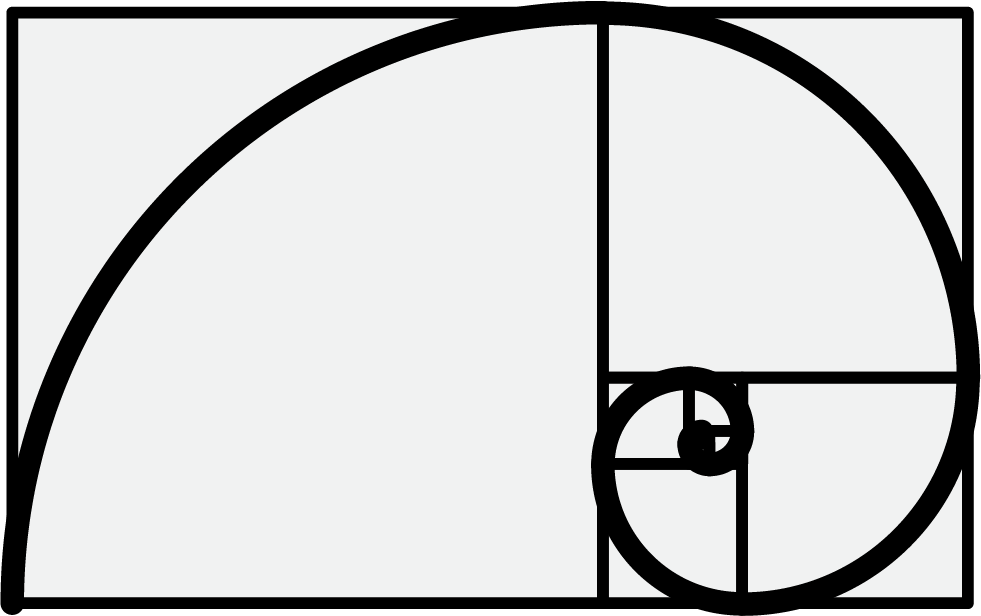
\includegraphics[height=0.75cm]{../../AAA_template_latex_settings/pwr-control_logo_doc.png}}
\lfoot{\href{http://www.pwr-control.com}{pwr-control.com}}
\cfoot{-\ \thepage\ -}
\rfoot{\textit{}}
\renewcommand{\headrulewidth}{0.4pt}
\renewcommand{\footrulewidth}{0.4pt}


\geometry{
	a4paper,
	top    = 2.5cm,
	bottom = 3.0cm,
	left   = 2.5cm,
	right  = 2.5cm
}

\hypersetup{
	colorlinks = true,
	urlcolor   = blue,
	linkcolor  = black,
	citecolor  = black
}

\pagenumbering{gobble}

\usetikzlibrary{decorations.pathreplacing,fit,shapes.geometric}
\usepackage[european,straightvoltages]{circuitikz}
\ctikzset{voltage dir=EF}

\newcommand{\ped}[1]{_{\mathrm{#1}}}
\newcommand{\code}[1]{\texttt{#1}}
\newcommand{\jj}{\mathrm{j}}
\newcommand{\dif}{\mathrm{d}}
\newcommand{\upu}{\,\mathrm{pu}}
\renewcommand{\tabularxcolumn}[1]{>{\raggedright\arraybackslash}p{#1}}
\setlength{\emergencystretch}{3em}
\sisetup{per-mode=symbol}
\DeclareSIUnit{\VA}{VA}

% ---------------- document metadata (read by the title page) ----------------
\newcommand{\DocCategory}{Technical Note}
\newcommand{\DocField}{Power Electronics and Control Systems}

\newcommand{\DocTitle}{%
	{\fontsize{20}{24}\selectfont\bfseries Parallel grid-forming modules} \\[16pt]
	{\fontsize{16}{20}\selectfont\bfseries power sharing, loss of the main grid, earthing and common mode}
}

\newcommand{\DocSubtitle}{%
	Design note of the model \code{pgfm\_ctrl\_analysis} (\code{grid-forming}, folder \code{parallel\_of\_GFMs}): the model as it runs today, what the literature offers, the first control version, implemented in the library block and tested on a companion model, the common mode of modules on one battery and the earthing of an industrial battery storage system.
}

\newcommand{\DocAuthor}{Davide Bagnara}
\newcommand{\DocRevision}{01}
\newcommand{\DocDate}{November 2026}

\newcommand{\DocAbstract}{%
	The model \code{pgfm\_ctrl\_analysis} puts three \SI{250}{\kilo\watt} active front ends in parallel on one lithium-ion battery and on a \SI{690}{\volt} grid emulator. Its purpose is the power sharing among grid-forming modules: in normal operation the modules follow the set-points of the plant; when the main grid is lost they keep the island alive and share the load, without any change of control mode. This note describes the model as it runs today, reviews what the group of M.~Liserre (Kiel University) and S.~Bolognani (ETH Z\"urich) offer for this problem, and gives the first control version: P--f droop with a low-pass filter and a lead term (a virtual synchronous machine with an inertia constant of \SI{1.25}{s}), Q--V droop, a virtual impedance in front of a voltage loop on the filter capacitor and of the existing current loop, current limitation and a time base distributed by PTP. Revision 01 replaces the virtual admittance of the first issue, which cannot hold an island of modules with LCL filters, analyses the small-signal stability of the whole discrete-time loop on stiff and weak grids and in the island, implements the control as the droop mode of the library block \code{grid\_forming\_dqctrl} and tests it on a light companion model: loss of the grid, load step, trip of a module, black start, clock errors and differences between the modules. It then treats the common mode of modules on one battery (common-mode chokes, PWM carriers aligned to a global PTP time, zero-sequence circulating currents), the earthing of an industrial battery energy storage system with the HF parasitic capacitances and earthing resistances now in the model, simulated for an unearthed, a high-resistance and a solidly earthed transformer star point, the residual current monitoring unit (RCMU) and the insulation monitor, and the step to three-level modules.
}

\newcommand{\RevisionHistory}{%
	00 & November 2026 & First issue: state of the model, literature, control proposal V1 and test plan, common mode and PTP alignment, earthing with the HF parameters of the model, RCMU and IMD, three-level outlook. & \DocAuthor \\
	01 & November 2026 & Control V1 reworked: virtual impedance in front of a voltage loop on the filter capacitor instead of the virtual admittance; small-signal analysis of the discrete-time loop; V1 as the droop mode of the library block \code{grid\_forming\_dqctrl}; companion model \code{pgfm\_droop} and results of the tests T0 to T5. & \DocAuthor \\
}

\newcommand{\MetaLabelA}{Project Repository}
\newcommand{\MetaValueAUrl}{https://github.com/pwr-control/grid-forming.git}
\newcommand{\MetaValueALabel}{grid-forming.git (parallel\_of\_GFMs)}

\newcommand{\MetaLabelB}{Framework}
\newcommand{\MetaValueB}{MATLAB/Simulink/Simscape}

\begin{document}

% =============================================================
%  pwr-control LaTeX template - FRONTESPIZIO
%
%  Da richiamare come prima istruzione dopo \begin{document}:
%      % =============================================================
%  pwr-control LaTeX template - FRONTESPIZIO
%
%  Da richiamare come prima istruzione dopo \begin{document}:
%      % =============================================================
%  pwr-control LaTeX template - FRONTESPIZIO
%
%  Da richiamare come prima istruzione dopo \begin{document}:
%      \input{../../AAA_template_latex_settings/titlepage}
%
%  Il documento deve definire prima di \begin{document}:
%      \DocCategory   categoria del documento
%      \DocField      area tecnica
%      \DocTitle      titolo (una o due righe)
%      \DocSubtitle   sottotitolo
%      \DocAuthor     autore/i, separati da virgola
%      \DocRevision   numero di revisione corrente (es. 00)
%      \DocDate       data della revisione corrente
%      \DocAbstract   abstract
%      \RevisionHistory  righe della tabella di revisione, nel formato
%                        Rev. & Date & Description & Authors \\
%      \MetaLabelA \MetaValueAUrl \MetaValueALabel
%      \MetaLabelB \MetaValueB
% =============================================================

\providecommand{\DocCategory}{Technical Research Report}
\providecommand{\DocField}{Power Electronics and Control Systems}
\providecommand{\DocSubtitle}{}
\providecommand{\DocRevision}{00}
\providecommand{\DocAbstract}{}
\providecommand{\RevisionHistory}{%
	\DocRevision & \DocDate & First issue. & \DocAuthor \\
}

\titlepage

% ---- Intestazione centrata ----
\begin{center}
	{\Large\scshape \DocCategory}\\[8pt]
	{\large\scshape \DocField}
\end{center}

\vspace{30pt plus 4pt minus 14pt}
\noindent\rule{\linewidth}{0.8pt}

% ---- Titolo ----
\begin{center}
	\DocTitle
\end{center}

\vspace{4pt}
\noindent\rule{\linewidth}{2.2pt}

% ---- Sottotitolo ----
\begin{center}
	\begin{onehalfspace}
		{\large\itshape \DocSubtitle}
	\end{onehalfspace}
\end{center}

% ---- Authors / Revision / Date ----
\vspace{30pt plus 4pt minus 14pt}

\noindent
\begin{minipage}[t]{0.46\linewidth}
	\raggedright
	\textbf{Authors:}\\[2pt]
	\DocAuthor
\end{minipage}%
\hfill
\begin{minipage}[t]{0.22\linewidth}
	\centering
	\textbf{Revision:}\\[2pt]
	\DocRevision
\end{minipage}%
\hfill
\begin{minipage}[t]{0.30\linewidth}
	\raggedleft
	\textbf{Date:}\\[2pt]
	\DocDate
\end{minipage}

\vspace{10pt}
\noindent\rule{\linewidth}{0.8pt}

% ---- Abstract ----
\vspace{24pt plus 4pt minus 12pt}

\begin{center}
	\begin{minipage}{0.88\linewidth}
		\footnotesize
		\begin{onehalfspace}
			\textbf{Abstract:} \DocAbstract
		\end{onehalfspace}
	\end{minipage}
\end{center}

\vfill

% ---- Revision history ----
\begin{center}
	\begin{minipage}{0.96\linewidth}
		\centering
		{\footnotesize\scshape Revision history}\\[6pt]
		{\footnotesize
			\begin{tabular}{@{}cl>{\raggedright\arraybackslash}p{0.36\linewidth}>{\raggedright\arraybackslash}p{0.28\linewidth}@{}}
				\toprule
				\textbf{Rev.} & \textbf{Date} & \textbf{Description} & \textbf{Authors} \\
				\midrule
				\RevisionHistory
				\bottomrule
			\end{tabular}}
	\end{minipage}
\end{center}

\vspace{18pt plus 4pt minus 10pt}

% ---- Metadati in fondo ----
\noindent
\begin{tabular}{@{} r @{\quad} l @{}}
	\textsc{\MetaLabelA:} & {\href{\MetaValueAUrl}{\MetaValueALabel}} \\[3pt]
	\textsc{\MetaLabelB:} & {\MetaValueB}       \\[3pt]
\end{tabular}

% =============================================================
%  Fine frontespizio
% =============================================================
\newpage
\pagenumbering{arabic}
\setcounter{page}{1}

%
%  Il documento deve definire prima di \begin{document}:
%      \DocCategory   categoria del documento
%      \DocField      area tecnica
%      \DocTitle      titolo (una o due righe)
%      \DocSubtitle   sottotitolo
%      \DocAuthor     autore/i, separati da virgola
%      \DocRevision   numero di revisione corrente (es. 00)
%      \DocDate       data della revisione corrente
%      \DocAbstract   abstract
%      \RevisionHistory  righe della tabella di revisione, nel formato
%                        Rev. & Date & Description & Authors \\
%      \MetaLabelA \MetaValueAUrl \MetaValueALabel
%      \MetaLabelB \MetaValueB
% =============================================================

\providecommand{\DocCategory}{Technical Research Report}
\providecommand{\DocField}{Power Electronics and Control Systems}
\providecommand{\DocSubtitle}{}
\providecommand{\DocRevision}{00}
\providecommand{\DocAbstract}{}
\providecommand{\RevisionHistory}{%
	\DocRevision & \DocDate & First issue. & \DocAuthor \\
}

\titlepage

% ---- Intestazione centrata ----
\begin{center}
	{\Large\scshape \DocCategory}\\[8pt]
	{\large\scshape \DocField}
\end{center}

\vspace{30pt plus 4pt minus 14pt}
\noindent\rule{\linewidth}{0.8pt}

% ---- Titolo ----
\begin{center}
	\DocTitle
\end{center}

\vspace{4pt}
\noindent\rule{\linewidth}{2.2pt}

% ---- Sottotitolo ----
\begin{center}
	\begin{onehalfspace}
		{\large\itshape \DocSubtitle}
	\end{onehalfspace}
\end{center}

% ---- Authors / Revision / Date ----
\vspace{30pt plus 4pt minus 14pt}

\noindent
\begin{minipage}[t]{0.46\linewidth}
	\raggedright
	\textbf{Authors:}\\[2pt]
	\DocAuthor
\end{minipage}%
\hfill
\begin{minipage}[t]{0.22\linewidth}
	\centering
	\textbf{Revision:}\\[2pt]
	\DocRevision
\end{minipage}%
\hfill
\begin{minipage}[t]{0.30\linewidth}
	\raggedleft
	\textbf{Date:}\\[2pt]
	\DocDate
\end{minipage}

\vspace{10pt}
\noindent\rule{\linewidth}{0.8pt}

% ---- Abstract ----
\vspace{24pt plus 4pt minus 12pt}

\begin{center}
	\begin{minipage}{0.88\linewidth}
		\footnotesize
		\begin{onehalfspace}
			\textbf{Abstract:} \DocAbstract
		\end{onehalfspace}
	\end{minipage}
\end{center}

\vfill

% ---- Revision history ----
\begin{center}
	\begin{minipage}{0.96\linewidth}
		\centering
		{\footnotesize\scshape Revision history}\\[6pt]
		{\footnotesize
			\begin{tabular}{@{}cl>{\raggedright\arraybackslash}p{0.36\linewidth}>{\raggedright\arraybackslash}p{0.28\linewidth}@{}}
				\toprule
				\textbf{Rev.} & \textbf{Date} & \textbf{Description} & \textbf{Authors} \\
				\midrule
				\RevisionHistory
				\bottomrule
			\end{tabular}}
	\end{minipage}
\end{center}

\vspace{18pt plus 4pt minus 10pt}

% ---- Metadati in fondo ----
\noindent
\begin{tabular}{@{} r @{\quad} l @{}}
	\textsc{\MetaLabelA:} & {\href{\MetaValueAUrl}{\MetaValueALabel}} \\[3pt]
	\textsc{\MetaLabelB:} & {\MetaValueB}       \\[3pt]
\end{tabular}

% =============================================================
%  Fine frontespizio
% =============================================================
\newpage
\pagenumbering{arabic}
\setcounter{page}{1}

%
%  Il documento deve definire prima di \begin{document}:
%      \DocCategory   categoria del documento
%      \DocField      area tecnica
%      \DocTitle      titolo (una o due righe)
%      \DocSubtitle   sottotitolo
%      \DocAuthor     autore/i, separati da virgola
%      \DocRevision   numero di revisione corrente (es. 00)
%      \DocDate       data della revisione corrente
%      \DocAbstract   abstract
%      \RevisionHistory  righe della tabella di revisione, nel formato
%                        Rev. & Date & Description & Authors \\
%      \MetaLabelA \MetaValueAUrl \MetaValueALabel
%      \MetaLabelB \MetaValueB
% =============================================================

\providecommand{\DocCategory}{Technical Research Report}
\providecommand{\DocField}{Power Electronics and Control Systems}
\providecommand{\DocSubtitle}{}
\providecommand{\DocRevision}{00}
\providecommand{\DocAbstract}{}
\providecommand{\RevisionHistory}{%
	\DocRevision & \DocDate & First issue. & \DocAuthor \\
}

\titlepage

% ---- Intestazione centrata ----
\begin{center}
	{\Large\scshape \DocCategory}\\[8pt]
	{\large\scshape \DocField}
\end{center}

\vspace{30pt plus 4pt minus 14pt}
\noindent\rule{\linewidth}{0.8pt}

% ---- Titolo ----
\begin{center}
	\DocTitle
\end{center}

\vspace{4pt}
\noindent\rule{\linewidth}{2.2pt}

% ---- Sottotitolo ----
\begin{center}
	\begin{onehalfspace}
		{\large\itshape \DocSubtitle}
	\end{onehalfspace}
\end{center}

% ---- Authors / Revision / Date ----
\vspace{30pt plus 4pt minus 14pt}

\noindent
\begin{minipage}[t]{0.46\linewidth}
	\raggedright
	\textbf{Authors:}\\[2pt]
	\DocAuthor
\end{minipage}%
\hfill
\begin{minipage}[t]{0.22\linewidth}
	\centering
	\textbf{Revision:}\\[2pt]
	\DocRevision
\end{minipage}%
\hfill
\begin{minipage}[t]{0.30\linewidth}
	\raggedleft
	\textbf{Date:}\\[2pt]
	\DocDate
\end{minipage}

\vspace{10pt}
\noindent\rule{\linewidth}{0.8pt}

% ---- Abstract ----
\vspace{24pt plus 4pt minus 12pt}

\begin{center}
	\begin{minipage}{0.88\linewidth}
		\footnotesize
		\begin{onehalfspace}
			\textbf{Abstract:} \DocAbstract
		\end{onehalfspace}
	\end{minipage}
\end{center}

\vfill

% ---- Revision history ----
\begin{center}
	\begin{minipage}{0.96\linewidth}
		\centering
		{\footnotesize\scshape Revision history}\\[6pt]
		{\footnotesize
			\begin{tabular}{@{}cl>{\raggedright\arraybackslash}p{0.36\linewidth}>{\raggedright\arraybackslash}p{0.28\linewidth}@{}}
				\toprule
				\textbf{Rev.} & \textbf{Date} & \textbf{Description} & \textbf{Authors} \\
				\midrule
				\RevisionHistory
				\bottomrule
			\end{tabular}}
	\end{minipage}
\end{center}

\vspace{18pt plus 4pt minus 10pt}

% ---- Metadati in fondo ----
\noindent
\begin{tabular}{@{} r @{\quad} l @{}}
	\textsc{\MetaLabelA:} & {\href{\MetaValueAUrl}{\MetaValueALabel}} \\[3pt]
	\textsc{\MetaLabelB:} & {\MetaValueB}       \\[3pt]
\end{tabular}

% =============================================================
%  Fine frontespizio
% =============================================================
\newpage
\pagenumbering{arabic}
\setcounter{page}{1}


\tableofcontents
\listoffigures
\listoftables
\newpage

\begin{onehalfspace}

% =============================================================
\section*{Nomenclature}
\addcontentsline{toc}{section}{Nomenclature}
\label{sec:nomenclature}

\begingroup % row colours of this table only: a \rowcolors left active breaks the multi-line TikZ nodes
\rowcolors{2}{tableShade}{white}
\begin{longtable}{@{} l p{0.74\linewidth} @{}}
	\toprule
	\textbf{Symbol} & \textbf{Meaning} \\
	\midrule
	\endfirsthead
	\toprule
	\textbf{Symbol} & \textbf{Meaning} \\
	\midrule
	\endhead
	\bottomrule
	\endfoot
	\bottomrule
	\endlastfoot
	AFE & active front end: three-phase PWM converter between a DC link and the AC network \\
	BESS, PCS & battery energy storage system; power conversion system (the converters of the BESS) \\
	GFM, GFL & grid-forming, grid-following \\
	VSM & virtual synchronous machine \\
	CM, ZSV, ZSCC & common mode; zero-sequence voltage; zero-sequence circulating current \\
	PTP & precision time protocol, IEEE 1588 \\
	IT, TN, HRG & earthing systems: not earthed (or through a high impedance), solidly earthed, earthed through a high resistance \\
	IMD & insulation monitoring device (IEC 61557-8) \\
	RCMU, RCD & residual current monitoring unit; residual current device \\
	$S\ped{b}$ & base power of a module, \SI{277.8}{\kilo\VA} (\SI{250}{\kilo\watt} at $\cos\varphi = 0.9$) \\
	$u\ped{bez}$, $i\ped{bez}$, $Z\ped{b}$ & base voltage and current (peak values) and base impedance of a module, \SI{563.4}{V}, \SI{328.7}{A}, \SI{1.714}{\ohm} \\
	$\omega\ped{b}$ & base angular frequency, $2\pi\cdot\SI{50}{Hz}$ \\
	$p$, $q$; $P\ped{f}$, $Q\ped{f}$ & active and reactive power of a module; the same after the low-pass filter (pu of $S\ped{b}$) \\
	$P^*$, $Q^*$ & set-points of a module from the plant controller \\
	$m\ped{p}$, $n\ped{q}$ & P--f and Q--V droop coefficients \\
	$m\ped{d}$ & gain of the lead term on the unfiltered power (damping of the swing modes) \\
	$E$, $U^*$ & amplitude of the internal voltage of a module; voltage set-point \\
	$X\ped{c,\mathit{k}}$, $\gamma_k$ & reactance of the connection of module $k$ to the common bus; gain error of its voltage measurement \\
	$\tau\ped{p}$, $\tau\ped{q}$ & time constants of the power filters \\
	$H$, $D$ & inertia constant and damping of the equivalent virtual synchronous machine \\
	$R\ped{v}$, $X\ped{v}$ & virtual resistance and reactance \\
	$r\ped{t}$, $\tau\ped{hp}$ & transient virtual resistance on the high-pass part of the output current; its time constant \\
	$u\ped{c}$, $i\ped{s}$ & voltage of the filter capacitor; converter current \\
	$u\ped{g}$, $i\ped{o}$ & voltage and current at the terminals of a module, after the grid-side inductor \\
	$u^*$, $i^*$ & references of the capacitor voltage and of the converter current \\
	$k\ped{pu}$, $k\ped{iu}$; $k\ped{pi}$, $k\ped{ii}$ & gains of the voltage PI; gains of the current PI \\
	$b$ & susceptance of the filter capacitor at \SI{50}{Hz} in pu, $\omega\ped{b} C\ped{F} Z\ped{b}$ \\
	$i\ped{max}$, $i\ped{thr}$ & current limit; threshold of the virtual-impedance current limitation \\
	$L$, $L_0$, $C\ped{F}$ & filter of a module: positive- and zero-sequence inductance of the three-phase inductor, filter capacitance \\
	$L_1$, $L_2$, $X_2$ & LCL filter of the library block: converter-side and grid-side inductors; reactance of $L_2$ \\
	$C\ped{pole}$, $C\ped{ac}$ & capacitance to earth of one battery pole, of one phase of the LV side \\
	$r\ped{gnd}$, $r\ped{star}$ & earthing resistor of one battery pole; resistance from the transformer star point to earth \\
\end{longtable}
\endgroup
\addtocounter{table}{-1}

% =============================================================
\section{Scope and summary}
\label{sec:scope}

The model \code{pgfm\_ctrl\_analysis} of the folder \path{parallel_of_GFMs} of the repository \code{grid-forming} has three AFE modules of \SI{250}{\kilo\watt} in parallel on one lithium-ion battery and on a \SI{690}{V}, \SI{1}{MVA} grid emulator. Its purpose is the study of the \emph{power sharing among grid-forming modules}: in normal operation the modules follow the set-points of the plant controller; if the main grid is lost, they must keep the voltage and the frequency of the island and share its load, ideally without detecting the event and without switching control mode. Two further topics belong to the same machine and are treated here because they decide what the power stage and the PWM must look like:

\begin{itemize}[nosep]
	\item the \emph{common mode} of modules that share one battery and one AC bus: common-mode chokes and PWM carriers aligned to a global time distributed by PTP;
	\item the \emph{earthing} of an industrial BESS: where the common-mode voltage of the bridges goes, which parasitic capacitances and earthing resistances to put in the model, how the insulation is monitored (IMD) and how the residual current is measured (RCMU).
\end{itemize}

The note proposes a first control version (V1) that can be implemented and simulated now, and a test plan to judge it. The main points are:

\begin{mybox}
	\textbf{Control V1 (Section~\ref{sec:v1}).} Every module is a voltage source behind a virtual impedance: P--f droop with a low-pass filter on the measured power and a lead term ($m\ped{p} = \SI{2}{\percent}$, $\tau\ped{p} = \SI{50}{ms}$, the same as a virtual synchronous machine with $H = \SI{1.25}{s}$ and $D = 50$), Q--V droop ($n\ped{q} = \SI{5}{\percent}$), a virtual impedance ($R\ped{v} = 0.05$, $X\ped{v} = \SI{0.10}{pu}$, and a transient resistance) that gives the reference of a voltage loop on the filter capacitor, in front of the existing current loop, a current limit of \SI{1.2}{pu} with a threshold virtual impedance, and the time base of the modules aligned by PTP. Rev.~01 replaces the virtual admittance of Rev.~00, which cannot hold an island of modules with LCL filters. There is no grid-loss detection and no mode change: on the loss of the grid the modules take the load at once and the frequency settles on the droop line (\SI{-0.24}{Hz} in the test case). The small-signal analysis of the whole discrete-time loop gives a damping ratio of 0.45 to 0.47 to the swing modes and of at least 0.39 to the electromagnetic modes, from a stiff grid to a weak grid and in the island. The reactive sharing is limited by the accuracy of the voltage measurements more than by the impedances, the active sharing by the clock errors if the time base is not aligned.

	\textbf{Implementation and tests (Sections~\ref{sec:routes} and~\ref{sec:tests}).} Done (route A): the control V1 is the droop mode of the library block \code{grid\_forming\_dqctrl}, and the companion model \code{pgfm\_droop} (three modules, local load, grid breaker) passes the tests: loss of the grid, load step and trip of a module in the island without loss of synchronism, sharing of $P$ and $Q$ within \SI{0.0001}{pu}, black start, peak converter current at most \SI{1.04}{pu}. Next (route B): the validated control into \code{pgfm\_ctrl\_analysis} for the common-mode and earthing studies, which need its switching details.

	\textbf{Earthing (Section~\ref{sec:earthing}).} Battery referenced to earth through a high impedance, LV side of the transformer not earthed (IT), insulation monitor, RCMU per PCS, inverter-duty transformer with an earthed screen. The simulation of the model with the new parameters shows why: with the star point not earthed the battery poles move by only \SI{90}{V} peak to peak; with the star point solidly earthed the battery carries the whole common-mode voltage of the bridges, \SI{1160}{V} peak to peak, and the earth current is seven times higher (\SI{4.4}{A} against \SI{0.64}{A} rms).
\end{mybox}

% =============================================================
\section{The model today}
\label{sec:model}

\subsection{Power stage}

Figure~\ref{fig:system} shows the model and Table~\ref{tab:system} its data. Each module is the AFE part of the original \code{afe\_abc\_inv\_psm} subsystem: a two-level bridge, a three-phase inductor and a star of filter capacitors with its star point floating. The three-phase inductor has $L = L_0 = \SI{500}{\micro\henry}$: its positive-sequence inductance is the filter inductance, its zero-sequence inductance makes it the common-mode choke of the module. There is no grid-side inductor in the modules: the capacitors of the three modules are on the same LV bus, and the grid-side inductance of the LCL filter is the one of the grid emulator (transformer \SI{5}{\percent} and source \SI{5}{\percent} on \SI{1}{MVA}). The DC side of the three modules is one battery, the block \code{battery\_1}, with the HF parasitics and the earthing resistors of Section~\ref{sec:earthing}.

\begin{figure}[H]
	\centering
	\begin{tikzpicture}[font=\footnotesize, >=Latex,
		blk/.style={draw, thick, rounded corners=2pt, minimum height=0.95cm, minimum width=2.5cm, align=center, fill=orange!15},
		gb/.style={draw, thick, rounded corners=2pt, align=center, fill=gray!10},
		nw/.style={draw, dashed, rounded corners=2pt, align=center, fill=blue!5, font=\scriptsize},
		new/.style={draw, thick, dashed, rounded corners=2pt, align=center, fill=green!8, font=\scriptsize}]
		% battery and DC bus
		\node[gb, minimum width=2.0cm, minimum height=3.4cm] (bat) at (0,0) {\code{battery\_1}\\lithium-ion\\\SI{1183}{V}\\pack of\\\SI{250}{\kilo\watt\hour}};
		\draw[very thick] (1.75,-2.0) -- (1.75,2.0) node[above, xshift=-3mm, font=\scriptsize] {DC bus};
		\draw[thick] (bat.east) -- (1.75,0);
		% modules
		\foreach \y/\n in {1.45/1, 0/2, -1.45/3} {
			\node[blk] (m\n) at (3.65,\y) {module \n: bridge,\\$L$, $L_0$, $C\ped{F}$};
			\draw[thick] (1.75,\y) -- (m\n.west);
			\draw[thick] (m\n.east) -- (6.0,\y);
		}
		% clocks and PWM carriers of the modules on the PTP time
		\node[draw, dashed, thick, rounded corners=4pt, yellow!50!black, fit=(m1)(m3), inner sep=0.15cm] (grp) {};
		\node[gb, minimum width=2.9cm, minimum height=0.6cm, fill=yellow!15] (ptp) at (3.65,2.85) {global timing (PTP)};
		\draw[->, dashed, thick, yellow!50!black] (ptp.south) -- (grp.north);
		% LV bus
		\draw[very thick] (6.0,-2.0) -- (6.0,2.0) node[above, xshift=5mm, font=\scriptsize] {LV bus \SI{690}{V}};
		% proposed breaker and load
		\node[new, minimum width=1.3cm, minimum height=0.7cm] (brk) at (7.2,0) {breaker\\(to add)};
		\draw[thick] (6.0,0) -- (brk.west);
		\node[new, minimum width=1.5cm, minimum height=0.7cm] (load) at (7.2,-1.6) {local load\\(to add)};
		\draw[thick] (6.0,-1.6) -- (load.west);
		% transformer
		\draw[thick] (brk.east) -- (8.45,0);
		\draw[thick] (8.8,0) circle (0.35);
		\draw[thick] (9.3,0) circle (0.35);
		\node[font=\scriptsize, align=center] at (9.05,0.85) {Dyn11, \SI{1}{MVA}\\$u_k = \SI{5}{\percent}$};
		% grid source
		\draw[thick] (9.65,0) -- (10.35,0);
		\node[gb, minimum width=1.3cm, minimum height=0.9cm] (grid) at (11.05,0) {grid\\$L\ped{grid}$, FRT};
		% earthing elements
		\node[nw] (hfb) at (0,-2.85) {HF and Ground Network:\\$C\ped{pole}$, $r\ped{gnd}$ per pole};
		\draw[dashed] (bat.south) -- (hfb.north);
		\draw (hfb.south) -- ++(0,-0.15) node[ground] {};
		\node[nw] (hft) at (10.5,-1.6) {LV star point:\\$r\ped{star} \parallel 3C\ped{ac}$};
		\draw[dashed] (8.8,-0.35) |- (hft.west);
		\draw (hft.south) -- ++(0,-0.15) node[ground] {};
	\end{tikzpicture}
	\captionsetup{width=0.92\textwidth, font=small}
	\caption[The model \code{pgfm\_ctrl\_analysis}.]{The model \code{pgfm\_ctrl\_analysis}: three modules on one battery and on the LV bus of the grid emulator. Blue: the earthing elements of Section~\ref{sec:earthing}; yellow: the clocks and the PWM carriers of the modules, aligned to the PTP time; green: the breaker and the local load that the tests of Section~\ref{sec:tests} need.}
	\label{fig:system}
\end{figure}

\begin{table}[H]
	\centering
	\captionsetup{width=0.9\textwidth, font=small}
	\caption{Data of the model (\code{init\_model.m}, November 2026).}
	\label{tab:system}
	\rowcolors{2}{tableShade}{white}
	\small
	\begin{tabularx}{0.95\textwidth}{@{} >{\raggedright\arraybackslash}p{0.40\textwidth} X @{}}
		\toprule
		\textbf{Item} & \textbf{Value} \\
		\midrule
		modules & 3, \SI{250}{\kilo\watt} each, $S\ped{b} = \SI{277.8}{\kilo\VA}$, \SI{690}{V}, \SI{50}{Hz} \\
		base values (per module) & $u\ped{bez} = \SI{563.4}{V}$, $i\ped{bez} = \SI{328.7}{A}$ (peaks), $Z\ped{b} = \SI{1.714}{\ohm}$ \\
		three-phase inductor & $L = L_0 = \SI{500}{\micro\henry}$ (0.092~pu), plus \SI{5}{\micro\henry} leakage \\
		filter capacitors & $C\ped{F} = \SI{200}{\micro\farad}$ in star, star point floating (0.108~pu, \SI{29.9}{\kilo\var}) \\
		DC link & \SI{7.2}{\milli\farad} per module, battery at \SI{1183}{V} (SOC 0.85) \\
		PWM and control & \SI{4}{kHz}, double update ($t\ped{s} = \SI{125}{\micro s}$), dead time \SI{3}{\micro s} \\
		solver step & $t\ped{c} = \SI{1}{\micro s}$ (fixed step) \\
		grid emulator & transformer Dyn11 690/\SI{690}{V}, \SI{1}{MVA}, $u_k = \SI{5}{\percent}$; source $L\ped{grid} = \SI{75.8}{\micro\henry}$ (\SI{5}{\percent}) \\
		battery & one pack of \SI{250}{\kilo\watt} at 1C, i.e.\ about \SI{250}{\kilo\watt\hour} \\
		scenario & modules at $i_\xi^* = \SI{-0.85}{pu}$ (\SI{734}{\kilo\watt} into the battery), FRT test 25.4 of VDE-AR-N 4110 at \SI{0.75}{s} for \SI{250}{ms}, reactive current step at \SI{1.335}{s}, \SI{1.75}{s} in total \\
		block budget & 994 non-virtual blocks of the 1000 allowed by the Home license \\
		\bottomrule
	\end{tabularx}
	\rowcolors{1}{white}{white}
\end{table}

\subsection{Control and timing}

The modules are grid-following today. Each one has a PLL, a current loop with resonant PI controllers ($k\ped{p} = 0.6$, $k\ped{i} = \SI{35}{s^{-1}}$), the fault ride-through logic of VDE-AR-N 4110 and a current reference set by the init ($i_\xi^* = \SI{-0.85}{pu}$, then the reactive-current steps after the fault). A zero-sequence term \code{u\_cm\_comp\_modN} for the parallel operation is enabled by \code{param.afe.ref.en\_parallel\_mode} (0 for module 1, $-1$ for modules 2 and 3).

The block \code{global timing} gives each module its own clock with a gain error (fields \code{time\_gain\_module\_N} of \code{param.afe.behav}: 1.0002, 1.0015, 0.9988, i.e.\ errors of 200 to \SI{1500}{ppm}, deliberately large) and aligns it to the master time through a compensation loop and a transmission delay of \SI{250}{\micro s}: this is the model of the time distribution by PTP. The PWM carriers of the modules run on the aligned time, with an optional phase shift (fields \code{pwm\_phase\_shift\_modN}, zero today: carriers aligned).

\subsection{What the model cannot do yet}

\begin{itemize}[nosep]
	\item The modules cannot form the grid: they follow the PLL angle and a current reference (the control V1 is in the library block, not yet in this model).
	\item There is no breaker between the LV bus and the grid emulator and no local load, so the loss of the grid cannot be simulated (the companion model of Section~\ref{sec:routes} has both).
	\item The battery is sized for one module while the three modules draw \SI{734}{\kilo\watt}; the DC-link capacitors start without voltage (inrush of the battery in the first milliseconds).
	\item Every new function must be paid with blocks: 994 of 1000.
\end{itemize}

% =============================================================
\section{What the modules must do}
\label{sec:requirements}

The requirements below are the ones the first version is judged against; the numbers are proposals.

\begin{enumerate}[label=R\arabic*., nosep]
	\item \textbf{On the grid}: each module follows its set-points $P^*$, $Q^*$ from the plant controller and, without anything added, gives inertia and a frequency response proportional to the frequency deviation (primary response).
	\item \textbf{Loss of the main grid}: the upstream breaker opens with a local load on the LV bus. No detection, no change of mode: the modules keep voltage and frequency (frequency within \SI{\pm 1}{Hz}, positive-sequence voltage within \SI{\pm 10}{\percent}) and share the load in proportion to their rating (error below \SI{5}{\percent} of $S\ped{b}$ for $P$, below \SI{10}{\percent} for $Q$).
	\item \textbf{Robust sharing}: the sharing must survive different impedances between the modules and the bus (cables, tolerances), the errors of the voltage measurements and the clock errors of the modules.
	\item \textbf{N$-$1}: the trip of one module in the island must not stop the others.
	\item \textbf{Current}: the converter current stays below \SI{1.2}{pu} in every event, the module stays grid-forming while it limits.
	\item \textbf{Later}: frequency and voltage restoration in the island, resynchronization and reconnection to the grid, fault ride-through as a grid-forming unit (GB grid code GC0137 style).
\end{enumerate}

% =============================================================
\section{Literature: Liserre, Bolognani and the base references}
\label{sec:literature}

\subsection{The group of M. Liserre (Kiel University)}

The Chair of Power Electronics of Kiel University has worked on grid-forming converters in parallel and in mixed plants, mostly in the frame of virtual synchronous machines:

\begin{itemize}[nosep]
	\item the review of Rosso, Wang, Liserre, Lu and Engelken \cite{rosso2021} classifies the grid-forming controls (droop, power synchronization, virtual synchronous machines, matching and oscillator-based controls), their inner loops (cascaded voltage and current loops, single loops, virtual impedance and admittance), their synchronization and their current limitation; it is the map used in this note to place the choice of Section~\ref{sec:choice};
	\item the robust stability of synchronverters (VSMs) operating in parallel \cite{rosso2019}, i.e.\ the case of this model, and of mixed plants with grid-forming and grid-following converters \cite{rosso2020}: the second one matters as soon as the modules share a bus with grid-following units (PV inverters, or the present modules);
	\item a battery storage system in grid-forming mode used to damp sub-synchronous oscillations \cite{zhou2022}: the same machine as here, seen from the grid;
	\item a current limitation strategy for grid-forming converters under symmetrical and asymmetrical faults that keeps the grid-forming behaviour before, during and after the fault, following the draft requirements of the British system operator and tested in power-hardware-in-the-loop \cite{kiel_curlim}: the reference for the fault ride-through of version 2;
	\item the zero-sequence circulating current of converters in parallel on a common DC link and a common AC side without transformers: Zhu, Liserre, Chen and Wu show that the third-order zero-sequence voltage injected by the space vector modulation drives it and propose a modulation that removes its effect \cite{zhu2017}; a further work analyses its spectrum and suppresses it with multi-resonant controllers \cite{kiel_zscc}. This is exactly the situation of the three modules on one battery (Section~\ref{sec:cm}).
\end{itemize}

\subsection{S. Bolognani (ETH Z\"urich) and the group of F. D\"orfler}

S.~Bolognani does not work on the inner control of a grid-forming converter but on the layer above it: how the set-points of many converters are computed so that the network is operated well. His results are the distributed control of the reactive power of the converters in a microgrid \cite{bolognani2013}, the distributed feedback control of the reactive power for voltage regulation and loss minimization \cite{bolognani2015}, and the online feedback optimization, in which an optimization algorithm runs as a controller driven by measurements rather than by a model of the network \cite{hauswirth2024}. For this model they are the natural \emph{tertiary} layer: the plant controller that computes $P^*$ and $Q^*$ (or the voltage set-points) of the modules from measurements, on top of the droop of each module.

In the same group, the grid-forming control with the strongest theoretical guarantees for converters in parallel is the dispatchable virtual oscillator control (dVOC) \cite{colombino2019}, which synchronizes the converters and shares the power with a single nonlinear law; the classic results on synchronization and power sharing of droop-controlled converters \cite{simpsonporco2013} and on the secondary frequency and voltage control by distributed averaging \cite{simpsonporco2015} are also from this school.

\subsection{Base references}

The droop control of converters in parallel goes back to Chandorkar, Divan and Adapa \cite{chandorkar1993}; the design of the output impedance for the sharing of parallel UPS inverters and the hierarchical (primary, secondary, tertiary) control of microgrids are due to Guerrero et al.\ \cite{guerrero2005, guerrero2011}; the synchronverter of Zhong and Weiss \cite{zhong2011} and the power-synchronization control of Zhang, Harnefors and Nee \cite{zhang2010} are the two other classic grid-forming laws; D'Arco and Suul \cite{darco2014} show that a droop with a low-pass filter on the power and a virtual synchronous machine are the same controller; Pogaku, Prodanovi\'c and Green \cite{pogaku2007} model and test the cascade of droops, virtual impedance, voltage loop on the filter capacitor and current loop in an inverter-based microgrid, and D'Arco, Suul and Fosso \cite{darco2015} build a virtual synchronous machine on the same cascade; Paquette and Divan \cite{paquette2015} limit the current of grid-forming inverters with a virtual impedance; Golsorkhi, Lu and Guerrero \cite{golsorkhi2017} replace the frequency droop with a common time reference (GPS) and an angle droop. The textbook of Teodorescu, Liserre and Rodr\'iguez \cite{teodorescu2011} covers the converter-level part. The grid-forming block of the library and its control are described in \cite{afe_note, gfm_note}; the effect of the PWM carriers of AFEs in parallel on the grid power quality in \cite{modularity_note}.

\subsection{Choice for the first version}
\label{sec:choice}

The first version uses the \textbf{droop with low-pass filter, equivalent to a virtual synchronous machine}, with a virtual impedance in front of a voltage loop on the filter capacitor and of the existing current loop:

\begin{itemize}[nosep]
	\item it is the structure most used in industry and in the grid codes for grid-forming units, and the one of the Kiel works on parallel VSMs \cite{rosso2019, rosso2021}; tuning it is tuning two physical numbers, inertia and droop;
	\item the sharing of active power in steady state is exact and needs no communication (it follows the droop coefficients); the sharing of reactive power is set by the droop and by the virtual impedance, which is chosen larger than the physical differences between the modules;
	\item it works in the same way on the grid and in the island: the loss of the grid is not an event for the control;
	\item the cascade keeps the existing current loop and its limitation; each module regulates the voltage of its own filter capacitor, and the virtual impedance with the grid-side inductor separates the modules on the bus, so that their voltage loops do not fight. Rev.~00 had chosen a virtual admittance in front of the current loop for fear of that fight; with LCL filters it leaves the voltage of an island to the resonance of the capacitors with the virtual inductors (Section~\ref{sec:whycascade});
	\item dVOC \cite{colombino2019} is the comparison for version 2; the online feedback optimization of Bolognani \cite{hauswirth2024} is the tertiary layer above the modules; with the PTP time in the plant the angle droop of \cite{golsorkhi2017} is an option that removes the frequency deviation.
\end{itemize}

% =============================================================
\section{Control V1: droop grid-forming modules with virtual impedance}
\label{sec:v1}

Rev.~00 of this note proposed a virtual admittance in front of the existing current loop. The analysis of the discrete-time loop of the block and the averaged simulation of three modules showed that this structure cannot hold an island formed by modules with LCL filters (Section~\ref{sec:whycascade}). Rev.~01 replaces it with the cascade of \cite{pogaku2007, darco2015}: the droops give the internal voltage, a virtual impedance gives the reference of the filter-capacitor voltage, a voltage loop on the capacitor gives the reference of the existing current loop. This control is now the droop mode of the library block \code{grid\_forming\_dqctrl} (\code{p.ctrl.droop = 1}) and has been tested on the companion model \code{pgfm\_droop} (Sections~\ref{sec:routes} and~\ref{sec:tests}).

\subsection{Structure}

Figure~\ref{fig:v1} shows the control of one module. All quantities are in pu of the module base; the frames use the amplitude-invariant transformation, so that $p$ and $q$ are in pu of $S\ped{b} = \tfrac32 u\ped{bez} i\ped{bez}$. $u\ped{c}$ is the voltage of the filter capacitor, $i\ped{s}$ the converter current, $u\ped{g}$ and $i\ped{o}$ the voltage and the current at the terminals of the module, after the grid-side inductor $L_2$. The measurements, the first-harmonic tracker, the current loop and the PWM are those of the block; the droop mode replaces its phase generator and its voltage loop.

\begin{figure}[H]
	\centering
	\begin{tikzpicture}[font=\footnotesize, >=Latex,
		blk/.style={draw, thick, rounded corners=2pt, minimum height=1.05cm, align=center, fill=orange!15},
		old/.style={draw, thick, rounded corners=2pt, minimum height=1.05cm, align=center, fill=gray!10}]
		\node[blk, text width=1.0cm] (pq) at (0,0) {power\\$p$, $q$\\LPF};
		\node[blk, text width=2.9cm] (pf) at (2.95,1.0) {P--f droop\\$\omega = 1 + m\ped{p}(P^* - P\ped{f})$\\$-\,m\ped{d}(p - P\ped{f})$};
		\node[blk, text width=2.9cm] (qv) at (2.95,-1.0) {Q--V droop\\$E = U^* + n\ped{q}(Q^* - Q\ped{f})$};
		\node[blk, text width=2.2cm] (int) at (6.35,1.0) {angle\\$\theta = \int \omega\ped{b}\,\omega\,\dif t$};
		\node[blk, text width=2.9cm] (vi) at (6.55,-1.0) {virtual impedance\\$u^* = E - Z\ped{v} i\ped{o} - r\ped{t}\, i\ped{o,hp}$};
		\node[blk, text width=2.1cm] (vl) at (9.85,-1.0) {voltage PI on $u\ped{c}$\\$+\,i\ped{o} + \jj b\, u\ped{c}$\\limit $i\ped{max}$};
		\node[old, text width=1.75cm] (cl) at (12.65,-1.0) {current loop\\$+\,u\ped{c}$\\(block)};
		\node[old, text width=1.9cm] (pwm) at (12.65,1.0) {SVPWM,\\carrier on PTP};
		\draw[->] ([yshift=0.3cm]pq.east) -- ++(0.3,0) |- node[pos=0.75, above] {$P\ped{f}$} (pf.west);
		\draw[->] ([yshift=-0.3cm]pq.east) -- ++(0.3,0) |- node[pos=0.75, below] {$Q\ped{f}$} (qv.west);
		\draw[->] (pf.east) -- node[above] {$\omega$} (int.west);
		\draw[->] (qv.east) -- node[above] {$E$} (vi.west);
		\draw[->] (vi.east) -- node[above] {$u^*$} (vl.west);
		\draw[->] (vl.east) -- node[above] {$i^*$} (cl.west);
		\draw[->] (cl.north) -- node[right] {$m$} (pwm.south);
		\draw[->] (int.north) -- ++(0,0.45) node[above, font=\scriptsize] {$\theta$ to all frames};
		\draw[<-] (pq.south) -- ++(0,-0.5) node[below] {$u\ped{g}$, $i\ped{o}$};
		\draw[<-] (vi.south) -- ++(0,-0.45) node[below] {$i\ped{o}$};
		\draw[<-] (vl.south) -- ++(0,-0.45) node[below] {$u\ped{c}$, $i\ped{o}$};
		\draw[<-] (cl.south) -- ++(0,-0.45) node[below] {$i\ped{s}$, $u\ped{c}$};
		\draw[<-] (pf.north) -- ++(0,0.4) node[above] {$P^*$};
		\draw[<-] (qv.south) -- ++(0,-0.45) node[below] {$Q^*$, $U^*$};
	\end{tikzpicture}
	\captionsetup{width=0.92\textwidth, font=small}
	\caption[Control V1 of one module.]{Control V1 of one module (Rev.~01). Orange: droop mode of the block; grey: parts of the block that the droop mode keeps. $Z\ped{v} = R\ped{v} + \jj X\ped{v}$, $i\ped{o,hp} = i\ped{o} - i\ped{o,lp}$ the high-pass part of the output current, $b$ the susceptance of the filter capacitor.}
	\label{fig:v1}
\end{figure}

\subsection{Power measurement}

With $u\ped{g}$ and $i\ped{o}$ in the frame of the module (angle $\theta$), sampled at the previous control step as everything in the block:
\begin{equation}
	p = u_{gd} i_{od} + u_{gq} i_{oq}, \qquad q = u_{gq} i_{od} - u_{gd} i_{oq}, \qquad
	\tau\ped{p}\,\dot P\ped{f} = p - P\ped{f}, \qquad \tau\ped{q}\,\dot Q\ped{f} = q - Q\ped{f}.
	\label{eq:power}
\end{equation}
These are the powers that the module delivers to the bus: the \SI{0.108}{pu} of reactive power of its own filter capacitor stay inside the module and do not enter the droop. The filters at $\tau\ped{p} = \tau\ped{q} = \SI{50}{ms}$ attenuate the \SI{100}{Hz} ripple of an unbalanced load by a factor 31.

\subsection{Active power: P--f droop with low-pass filter and lead term, a virtual synchronous machine}

The frequency of the module and its angle are
\begin{equation}
	\omega = 1 + \Delta\omega^* + m\ped{p}\,(P^* - P\ped{f}) - m\ped{d}\,(p - P\ped{f}), \qquad \dot\theta = \omega\ped{b}\,\omega ,
	\label{eq:pf}
\end{equation}
with $P^*$ and the frequency offset $\Delta\omega^*$ from the plant controller. Without the lead term, eliminating $P\ped{f}$ with (\ref{eq:power}) gives, for constant set-points,
\begin{equation}
	\frac{\tau\ped{p}}{m\ped{p}}\,\dot\omega = P^* - p - \frac{1}{m\ped{p}}\,(\omega - 1)
	\quad\Longleftrightarrow\quad
	2H\,\dot\omega = P^* - p - D\,(\omega - 1),
	\label{eq:vsm}
\end{equation}
the swing equation of a synchronous machine with $2H = \tau\ped{p}/m\ped{p}$ and $D = 1/m\ped{p}$ \cite{darco2014}. With $m\ped{p} = 0.02$ (\SI{1}{Hz} for \SI{1}{pu} of power) and $\tau\ped{p} = \SI{50}{ms}$: $H = \SI{1.25}{s}$, $D = 50$. The lead term on the unfiltered power ($m\ped{d} = 0.01$) damps the swing modes without changing the droop, the steady state or the inertia seen by slow disturbances: without it the swing modes have a damping ratio of 0.15 (Table~\ref{tab:smallsignal}). In steady state all modules run at the same frequency, so $P^*_k - P_k = (\omega - 1)/m\ped{p}$ is the same for all: with equal $m\ped{p}$ and $P^*$ the modules share the active power exactly, whatever their impedance.

\subsection{Reactive power: Q--V droop}

The amplitude of the internal voltage is
\begin{equation}
	E = U^* + n\ped{q}\,(Q^* - Q\ped{f}), \qquad n\ped{q} = 0.05 ,
	\label{eq:qv}
\end{equation}
$U^*$ the voltage set-point (\SI{1}{pu} plus an offset from the plant controller). Unlike the frequency, the voltage is not the same at every module. The converter-side inductor $L_1$ is inside the loops and does not count; module $k$ is its internal voltage behind the virtual impedance, its grid-side inductor ($X_2 = \SI{0.015}{pu}$) and the reactance $X\ped{c,\mathit{k}}$ of its connection to the common bus (cable, busbar), and its reactive power is about
\begin{equation}
	Q_k \simeq \frac{U^* + n\ped{q} Q^*_k - (1 + \gamma_k)\,U - R\ped{v} P_k}{X\ped{v} + X_2 + X\ped{c,\mathit{k}} + n\ped{q}} ,
	\label{eq:qshare}
\end{equation}
$U$ the bus voltage and $\gamma_k$ the gain error of the voltage measurement of the module. With $X\ped{v} = \SI{0.10}{pu}$ and $n\ped{q} = 0.05$ the denominator is \SI{0.165}{pu}: a connection \SI{0.01}{pu} longer (\SI{55}{\micro\henry}) takes \SI{6}{\percent} of the reactive power of the module, a gain error of \SI{1}{\percent} moves its reactive power by $\gamma U/0.165 = \SI{0.056}{pu}$ of $S\ped{b}$: in the island the accuracy of the voltage measurement, not the impedances, sets the reactive sharing (test T4). The term $R\ped{v} P_k$ couples the active power into the reactive one: a module that delivers $\Delta P$ more than the others takes $\Delta Q \simeq -R\ped{v}\Delta P/0.165 = -0.3\,\Delta P$ (test T1); with equal set-points it has no effect.

\subsection{Virtual impedance, voltage loop and current loop}

The reference of the capacitor voltage is the internal voltage $e = (E, 0)$ in the frame $\theta$ minus the drop on a virtual impedance:
\begin{equation}
	u^* = E - (R\ped{v} + \jj X\ped{v})\, i\ped{o} - r\ped{t}\,(i\ped{o} - i\ped{o,lp}), \qquad \tau\ped{hp}\,\dot i\ped{o,lp} = i\ped{o} - i\ped{o,lp} .
	\label{eq:vi}
\end{equation}
$X\ped{v} = \SI{0.10}{pu}$ (\SI{0.55}{mH}) dominates the physical differences between the modules and decouples $P$ from $Q$; $R\ped{v} = \SI{0.05}{pu}$ (\SI{86}{\milli\ohm}) and the transient resistance $r\ped{t} = \SI{0.15}{pu}$ on the high-pass part of $i\ped{o}$ ($\tau\ped{hp} = \SI{5}{ms}$, no effect in steady state) damp the electromagnetic modes. The impedance is quasi-static, the product $\jj X\ped{v} i\ped{o}$ in the frame without the derivative of $i\ped{o}$, so that no measured current is differentiated.

A vector PI in the frame regulates the capacitor voltage, with the feedforward of the output current and of the capacitor current at the fundamental:
\begin{equation}
	i^* = k\ped{pu}\,(u^* - u\ped{c}) + k\ped{iu}\!\int (u^* - u\ped{c})\,\dif t + i\ped{o} + \jj\, b\, u\ped{c}, \qquad |i^*| \le i\ped{max},
	\label{eq:vloop}
\end{equation}
$b = \omega\ped{b} C\ped{F} Z\ped{b} = \SI{0.108}{pu}$, $k\ped{pu} = 0.8$, $k\ped{iu} = \SI{80}{s^{-1}}$; the limiter clips on a circle and holds the integrators while it clips. The current loop of the block follows $i^*$ and receives $u\ped{c}$ as feedforward of the modulation index, so that its PI only corrects the drop on $L_1$:
\begin{equation}
	m = k\ped{pi}\,(i^* - i\ped{s}) + k\ped{ii}\!\int (i^* - i\ped{s})\,\dif t + \frac{u\ped{c}}{k\ped{m}}, \qquad k\ped{m} = \frac{u\ped{dc}}{\sqrt3\, u\ped{bez}},
	\label{eq:cl}
\end{equation}
with the gains of the block ($k\ped{pi} = 0.75$, $k\ped{ii} = \SI{35}{s^{-1}}$) and $u\ped{dc}$ the acquired DC-link voltage.

\subsection{Why a cascade and not the virtual admittance of Rev.~00}
\label{sec:whycascade}

\paragraph{Virtual admittance with LCL modules.} In Rev.~00 the internal voltage drove a virtual inductor towards the measured voltage and its current was the reference of the current loop: each module was a current source behind a virtual admittance. With LCL filters the filter capacitors of the modules are on the bus, and in the island nothing else sets its voltage: the bus is a resonant circuit of the capacitors and the virtual inductors, damped by $R\ped{v}$ alone, and the delays of the voltage measurement and of the current loop make it unstable. In the averaged model of the three modules (ideal current loop with a lag of \SI{0.4}{ms}, voltage measurement filtered at \SI{2}{ms}) the structure holds the operation on the grid, but after the loss of the grid the bus voltage oscillates between 0.5 and \SI{3.9}{pu} within \SI{0.4}{s} and the currents run into the limit; with faster measurements (\SI{0.1}{ms}) it is unstable already on the grid. A grid-forming module with an LCL filter must regulate the voltage of its own capacitor.

\paragraph{Feedforward of the output current.} Without the feedforward of $i\ped{o}$ in (\ref{eq:vloop}) the voltage PI alone must supply the whole output current, its integrator becomes the slowest element of the chain and the swing mode is unstable on every grid ($\zeta = -0.28$ at \SI{2.4}{Hz}, Table~\ref{tab:smallsignal}): on a stiff grid the module slips. With the feedforward the PI only corrects the errors, the capacitor voltage follows $u^*$ within a few milliseconds and the module is the voltage source that the droop assumes. The voltage PI of the block ($k\ped{pu} = 0.5$, $k\ped{iu} = \SI{18}{s^{-1}}$) is stable with the feedforward but leaves the swing modes at $\zeta = 0.23$; $k\ped{pu} = 0.8$, $k\ped{iu} = \SI{80}{s^{-1}}$ give 0.45.

\subsection{Current limitation}

Two stages. Above $|i\ped{o}| = i\ped{thr} = \SI{1.0}{pu}$ a threshold virtual impedance \cite{paquette2015} adds $\Delta X\ped{v} = k_X(|i\ped{o}| - i\ped{thr})$ with $k_X = 1$ and $\Delta R\ped{v} = \Delta X\ped{v}/5$, so that the module stays a voltage source behind a larger impedance; the reference of the current loop is clipped on a circle of radius $i\ped{max} = \SI{1.2}{pu}$ with the integrators of the voltage PI held (anti-windup). While the module limits, the measured power is lower than the one it would deliver and the droop raises its frequency: in version 1 this is accepted (it is what makes an overloaded module shed load to the others); the fault ride-through with a frozen or bounded frequency is version 2 \cite{kiel_curlim}.

\subsection{Start, synchronization, black start and loss of the grid}

Until $t\ped{sync}$ (\SI{0.05}{s} in the example parameters of the block, \SI{0.1}{s} in the companion model) the module follows the terminal voltage: its angle is that of the first-harmonic tracker of $u\ped{g}$, turned onto the sampled capacitor voltage with a time constant of \SI{5}{ms}, its current reference is zero and the power filters and the low-pass filter of $i\ped{o}$ run. At $t\ped{sync}$ the droop starts from that angle and that operating point without a step, and the set-points $P^*$, $Q^*$ ramp from zero in $t\ped{ramp} = \SI{0.1}{s}$. The turn matters: the output of the tracker leads the samples of the previous trigger by about \SI{0.07}{rad}, and a voltage loop started in its frame pulls $u\ped{c}$ forward by as much, a kick of about \SI{0.3}{pu} of active power on the grid that the droop then takes back with a dip of \SI{0.13}{Hz}. If the bus is dead at $t\ped{sync}$ (tracker output below \SI{0.5}{pu}) the module makes a black start: its angle runs free from $\theta_0$ and $E$ ramps from zero in $t\ped{ramp}$; modules that black-start together synchronize through the droop, whatever their initial angles. On the loss of the grid nothing changes in the control: the modules, which were voltage sources, take the power that the grid supplied; the frequency moves with the inertia $2H$ and settles at the droop value. The plant controller (version 2) restores the frequency and the voltage, synchronizes the island to the grid when it comes back and closes the breaker.

\subsection{Small-signal analysis}
\label{sec:smallsignal}

Rev.~00 checked the power loops with the swing equation (\ref{eq:vsm}) of a module seen as an ideal voltage source behind $X\ped{v}$. Rev.~01 linearizes the whole discrete-time loop of the block: three modules with their LCL filters, the bus with the local load ($R$ in parallel with $L$ and its series resistance), the grid behind $R + L$, and the control of each module as in the block at $t\ped{s} = \SI{125}{\micro\second}$, with the one-step delay of the samples, the filters, the droops, the virtual impedance, the two PIs with their feedforwards and the modulation. The map $z_{k+1} = F(z_k)$ is written in a frame rotating at \SI{50}{Hz}; its equilibrium is found by Newton's method, its Jacobian by central differences, and each eigenvalue $\lambda$ gives $s = \ln\lambda / t\ped{s}$. Table~\ref{tab:smallsignal} gives the least-damped mode in two bands: the swing modes of the droops (below \SI{20}{Hz}) and the electromagnetic modes of the voltage loops with the filters and the network (20 to \SI{500}{Hz}), for a stiff grid ($X\ped{grid} = \SI{0.01}{pu}$), the grid of the model (\SI{10}{\percent} on \SI{1}{MVA}, \SI{0.028}{pu}), a weak grid ($X\ped{grid} = \SI{0.11}{pu}$, short-circuit ratio 3 for the three modules) and the island; the load is \SI{600}{\kilo\watt} + \SI{200}{\kilo\var}, $P^* = \SI{0.4}{pu}$.

\begin{table}[H]
	\centering
	\captionsetup{width=0.95\textwidth, font=small}
	\caption{Least-damped modes of the discrete-time loop of three modules: damping ratio $\zeta$ and frequency, swing modes (below \SI{20}{Hz}) and electromagnetic modes (20 to \SI{500}{Hz}).}
	\label{tab:smallsignal}
	\rowcolors{2}{tableShade}{white}
	\footnotesize
	\begin{tabularx}{\textwidth}{@{} >{\raggedright\arraybackslash}p{0.22\textwidth} l *{4}{>{\centering\arraybackslash}X} @{}}
		\toprule
		\textbf{Design} & \textbf{Modes} & \textbf{stiff grid} & \textbf{grid of the model} & \textbf{weak grid, SCR 3} & \textbf{island} \\
		\midrule
		V1, \SI{690}{V} module & swing & 0.45, \SI{5.6}{Hz} & 0.46, \SI{5.6}{Hz} & 0.47, \SI{5.5}{Hz} & 0.47, \SI{5.3}{Hz} \\
		 & electromagnetic & 0.61, \SI{75}{Hz} & 0.56, \SI{68}{Hz} & 0.39, \SI{56}{Hz} & 0.64, \SI{80}{Hz} \\
		V1, \SI{400}{V} example of the block & swing & 0.43, \SI{5.4}{Hz} & 0.44, \SI{5.3}{Hz} & 0.45, \SI{5.2}{Hz} & 0.46, \SI{5.1}{Hz} \\
		 & electromagnetic & 0.41, \SI{61}{Hz} & 0.39, \SI{59}{Hz} & 0.30, \SI{55}{Hz} & 0.43, \SI{62}{Hz} \\
		without $r\ped{t}$ & electromagnetic & 0.07, \SI{86}{Hz} & 0.07, \SI{86}{Hz} & 0.07, \SI{86}{Hz} & 0.07, \SI{86}{Hz} \\
		without $m\ped{d}$ & swing & 0.14, \SI{4.9}{Hz} & 0.14, \SI{4.8}{Hz} & 0.15, \SI{4.8}{Hz} & 0.16, \SI{4.7}{Hz} \\
		voltage PI of the block (0.5, \SI{18}{s^{-1}}) & swing & 0.23, \SI{5.1}{Hz} & 0.23, \SI{5.1}{Hz} & 0.24, \SI{5.0}{Hz} & 0.25, \SI{4.9}{Hz} \\
		without feedforward of $i\ped{o}$ & swing & $-0.29$, \SI{2.4}{Hz} & $-0.28$, \SI{2.4}{Hz} & $-0.27$, \SI{2.4}{Hz} & $-0.25$, \SI{2.3}{Hz} \\
		\bottomrule
	\end{tabularx}
	\rowcolors{1}{white}{white}
\end{table}

With the parameters of Table~\ref{tab:v1param} the least-damped mode has $\zeta = 0.39$ (weak grid, \SI{56}{Hz}) for the \SI{690}{V} module and 0.30 for the \SI{400}{V} example of the block (\SI{330}{\micro\henry}, \SI{360}{\micro\farad}, \SI{80}{\micro\henry}), whose parameter file carries the same values. A light island load (\SI{0.3}{pu}) or $P^* = \SI{1}{pu}$ change the damping by less than 0.02. The electromagnetic modes between 55 and \SI{86}{Hz} are those of the voltage loops with the filter and the network; the transient resistance $r\ped{t}$ takes them from 0.07 to 0.4--0.6. The swing modes at about \SI{5.5}{Hz} owe their damping to the lead term and to the speed of the voltage loop. The expected values of Rev.~00 for the tests ($\zeta = 0.38$ on the grid and 0.28 in the island, from the swing equation alone) are replaced by these.

\subsection{Clock errors, PTP and power sharing}
\label{sec:clock}

The droop (\ref{eq:pf}) is computed on the time of the module. If its clock runs fast by $\varepsilon$, the frequency that the module believes to impose is wrong by $\varepsilon$, and in steady state, where all modules have the same real frequency,
\begin{equation}
	P_k = P^*_k - \frac{\omega - 1 - \varepsilon_k}{m\ped{p}}
	\quad\Rightarrow\quad
	P_j - P_k = \frac{\varepsilon_j - \varepsilon_k}{m\ped{p}} .
	\label{eq:clock}
\end{equation}
With the gains of the model, modules 2 and 3 are \SI{2700}{ppm} apart: without the time alignment they share with an error of \SI{13.5}{\percent} of $S\ped{b}$ (test T0: \SI{0.1345}{pu}); a \SI{50}{ppm} crystal gives \SI{0.25}{\percent} per module. The alignment of the clocks by PTP (the \code{global timing} of the model, the alignment loop of the block) removes this error (T0: \SI{0.0003}{pu}) and is the condition for the angle droop of version 2. The same time base aligns the PWM carriers (Section~\ref{sec:cm}).

\subsection{Parameters of V1}

\begin{table}[H]
	\centering
	\captionsetup{width=0.95\textwidth, font=small}
	\caption{Parameters of the control V1 (pu of the module base) and fields of \code{p.ctrl} of the block.}
	\label{tab:v1param}
	\rowcolors{2}{tableShade}{white}
	\footnotesize
	\begin{tabularx}{\textwidth}{@{} >{\raggedright\arraybackslash}p{0.27\textwidth} >{\raggedright\arraybackslash}p{0.17\textwidth} >{\raggedright\arraybackslash}p{0.21\textwidth} X @{}}
		\toprule
		\textbf{Parameter} & \textbf{Value} & \textbf{Field} & \textbf{Note} \\
		\midrule
		P--f droop $m\ped{p}$ & 0.02 & \code{droop\_mp} & \SI{1}{Hz} per pu; $D = 50$ \\
		power filters $\tau\ped{p}$, $\tau\ped{q}$ & \SI{50}{ms} & \code{droop\_tau\_p}, \code{\_q} & $H = \SI{1.25}{s}$ \\
		lead term $m\ped{d}$ & 0.01 & \code{droop\_md} & damping of the swing modes \\
		Q--V droop $n\ped{q}$ & 0.05 & \code{droop\_nq} & \\
		virtual impedance $R\ped{v}$, $X\ped{v}$ & 0.05, 0.10 & \code{droop\_rv}, \code{\_xv} & \SI{86}{\milli\ohm}, \SI{0.55}{mH} \\
		transient resistance $r\ped{t}$, $\tau\ped{hp}$ & 0.15, \SI{5}{ms} & \code{droop\_rt}, \code{\_tau\_hp} & damping of the electromagnetic modes, no effect in steady state \\
		threshold virtual impedance & $i\ped{thr} = 1.0$, $k_X = 1$, $X/R = 5$ & \code{droop\_i\_thr}, \code{\_kx}, \code{\_x\_r} & \cite{paquette2015} \\
		current limit $i\ped{max}$ & 1.2 & \code{droop\_i\_max} & clip of $i^*$, integrators held \\
		voltage PI $k\ped{pu}$, $k\ped{iu}$ & 0.8, \SI{80}{s^{-1}} & \code{droop\_kp\_u}, \code{\_ki\_u} & feedforward of $i\ped{o}$ and $\jj b u\ped{c}$ \\
		current loop $k\ped{pi}$, $k\ped{ii}$ & 0.75, \SI{35}{s^{-1}} & \code{kp\_i}, \code{ki\_i} & of the block, feedforward of $u\ped{c}$ \\
		start $t\ped{sync}$, $t\ped{ramp}$ & 0.05 (0.1), \SI{0.1}{s} & \code{droop\_t\_sync}, \code{\_t\_ramp} & 0.1 in the companion model \\
		set-points $P^*$, $Q^*$, $U^*$ & 0.4, 0, 1 & \code{droop\_p\_ref}, \code{\_q\_ref}, \code{ug\_ref} & offsets from the input \code{sync}: $[-;\,\Delta P^*;\,\Delta Q^*;\,\Delta U^*;\,\Delta\omega^*]$ \\
		time base & PTP & \code{k\_time}, \code{kp\_align}, \code{ki\_align} & clocks and carriers aligned \\
		\bottomrule
	\end{tabularx}
	\rowcolors{1}{white}{white}
\end{table}

\subsection{How V1 is put in the models}
\label{sec:routes}

\paragraph{Route A (done in Rev.~01): library block and a light model.} The control V1 is the droop mode of the MATLAB Function of the library block \code{grid\_forming\_dqctrl} \cite{afe_note} (\code{p.ctrl.droop = 1}, fields \code{droop\_*}; \code{ctrl\_log} from 43 to 55 signals, 44 to 55 for the droop; the input \code{sync} carries the set-point offsets; the ports do not change and the existing models are not affected). The block with the delta capacitors, \code{grid\_forming\_dqctrl\_delta}, links the same code. The companion model \code{pgfm\_droop.slx} in \path{parallel_of_GFMs/power_sharing} has three such blocks with the switching bridge, each on an ideal DC source, a switch in the output of each module (trip, with an RC snubber across each pole that takes the current of $L_2$ when it opens, as the arc of a contactor does until the current zero) and an optional cable, the \SI{690}{V} bus with the local load and a switched load step, and the grid (\SI{10}{\percent} on \SI{1}{MVA}) behind a breaker: 277 blocks, Simscape Foundation only, built by \code{build\_pgfm\_droop.m}, parameters and cases in \code{init\_pgfm\_droop.m}, tests in \code{pgfm\_droop\_tests.m}. It simulates about \SI{0.7}{s} per minute on a desktop PC. The battery with its earthing network and the grid emulator are not in it: common mode and earthing stay with route B.

\paragraph{Route B: the present model.} In \code{pgfm\_ctrl\_analysis} the PLL and the reference chain of each module (about 60 non-virtual blocks) are replaced by one MATLAB Function with the control V1, in front of the existing current loops; the blocks saved pay for the breaker and the load. It keeps the switching details, the PTP model and the common-mode paths, but it changes the control of the modules that the model was built around, and the license limit stays tight.

The two routes are complementary: A to design and validate the control, B afterwards to study common mode, earthing and PTP with the validated control.

\subsection{Tests on the companion model}
\label{sec:tests}

Module of \SI{250}{\kilo\watt} at \SI{690}{V} ($S\ped{b} = \SI{277.8}{\kilo\VA}$), $L_1 = \SI{500}{\micro\henry}$, $C\ped{F} = \SI{200}{\micro\farad}$, $L_2 = \SI{80}{\micro\henry}$, $u\ped{dc} = \SI{1070}{V}$, PWM at \SI{4}{kHz} with double update, solver step \SI{1}{\micro\second}; local load \SI{600}{\kilo\watt} + \SI{200}{\kilo\var} at \SI{690}{V} (constant impedance), $P^* = \SI{0.4}{pu}$, $Q^* = 0$. On the grid the breaker closes at \SI{1}{ms} and the modules synchronize until \SI{0.1}{s}. Table~\ref{tab:tests} gives the events and the results; the frequency is that of the phase generators, the voltage $|u|$ the magnitude of the bus voltage averaged over \SI{1}{ms}, the rate of change of frequency the largest derivative of the frequency averaged over \SI{10}{ms}, from 10 to \SI{200}{ms} after the event, the settling time the time to enter a band of \SI{\pm 0.01}{pu} around the final $P\ped{f}$.

\begin{table}[H]
	\centering
	\captionsetup{width=0.97\textwidth, font=small}
	\caption{Tests of the control V1 on \code{pgfm\_droop} (powers in pu of $S\ped{b}$, per module).}
	\label{tab:tests}
	\rowcolors{2}{tableShade}{white}
	\footnotesize
	\begin{tabularx}{\textwidth}{@{} l >{\raggedright\arraybackslash}p{0.30\textwidth} X @{}}
		\toprule
		\textbf{Test} & \textbf{Event} & \textbf{Result} \\
		\midrule
		T0 & island (black start); clocks of the modules \num{1.0002}, \num{1.0015}, \num{0.9988}; time alignment off, then on & off: $P$ = 0.639, 0.704, \SI{0.569}{pu}, spread \SI{0.1345}{pu} as (\ref{eq:clock}); on: spread \SI{0.0003}{pu} \\
		T1 & on the grid: $P^*$ of module 1 from 0.4 to \SI{0.8}{pu} at \SI{0.6}{s} & $P\ped{f}$ of module 1 settles in \SI{0.17}{s}, overshoot \SI{5}{\percent}; its frequency steps by $m\ped{p}\,\Delta P^* = \SI{0.4}{Hz}$ and comes back to \SI{50}{Hz}; $P = P^*$ within \SI{0.0001}{pu}; $Q$ of module 1 \SI{-0.14}{pu} (\ref{eq:qshare}: $-0.12$, the rest is the angle across $X\ped{v}$); peak current \SI{1.04}{pu} \\
		T2 & loss of the grid at \SI{1.0}{s}, \SI{600}{\kilo\watt} + \SI{200}{\kilo\var} on the bus & \num{50.000} to \SI{49.762}{Hz} (nadir 49.758), \SI{4.6}{Hz/s}; $|u|$ 0.978 to \SI{0.926}{pu}, minimum \SI{0.82}{pu}; $P$ 0.40 to \SI{0.638}{pu} and $Q$ to \SI{0.204}{pu} each, settled in \SI{0.15}{s}, overshoot \SI{0.1}{\percent}; peak current \SI{0.72}{pu} \\
		T3 & island: load step of +\SI{150}{\kilo\watt} at \SI{1.5}{s} (after T2) & to \SI{49.623}{Hz} (nadir 49.617), \SI{2.7}{Hz/s}; $|u|$ to \SI{0.917}{pu}, minimum \SI{0.85}{pu}; $P$ to \SI{0.777}{pu} and $Q$ \SI{0.201}{pu} each, settled in \SI{0.13}{s}; spread of $P$ and $Q$ below \SI{0.0001}{pu}; peak current \SI{0.86}{pu} \\
		T4 & island (black start): module 3 with $L_1$ + \SI{20}{\percent}; with a cable of \SI{0.01}{pu}; with $U^*$ \SI{1}{\percent} low (a gain error of \SI{1}{\percent}) & spread of $Q$: \SI{0.002}{pu} (no effect); \SI{0.011}{pu} (\ref{eq:qshare}: 0.012); \SI{0.058}{pu} (\ref{eq:qshare}: 0.056; Rev.~00 expected 0.045). $P$ shared within \SI{0.0001}{pu} in the three cases \\
		T5 & \SI{450}{\kilo\watt} + \SI{150}{\kilo\var}: loss of the grid at \SI{1.0}{s}, trip of module 3 at \SI{1.5}{s} & loss of the grid: \SI{49.903}{Hz}, $P$ 0.40 to \SI{0.497}{pu}; trip: modules 1 and 2 to $P = \SI{0.704}{pu}$, $Q = \SI{0.224}{pu}$ at \SI{49.696}{Hz} (nadir 49.689, \SI{3.3}{Hz/s}), minimum voltage \SI{0.84}{pu}, settled in \SI{0.15}{s}, peak current \SI{0.79}{pu}; module 3 runs on at no load \\
		black start & no grid, \SI{600}{\kilo\watt} + \SI{200}{\kilo\var}, start at \SI{0.1}{s} & bus voltage at \SI{90}{\percent} in \SI{0.09}{s}, overshoot \SI{1.4}{\percent}; \SI{49.762}{Hz}, $P$ = \SI{0.638}{pu}, $Q$ = \SI{0.204}{pu} each, peak current \SI{0.71}{pu} \\
		\bottomrule
	\end{tabularx}
	\rowcolors{1}{white}{white}
\end{table}

All cases pass the checks of \code{pgfm\_droop\_tests.m}: equal sharing in the island (spread below \SI{0.01}{pu} of $P$ and \SI{0.02}{pu} of $Q$, except where the test introduces a difference), $P = P^*$ on the grid, frequency on the droop line, damped power (peak to peak of $P\ped{f}$ below \SI{0.02}{pu} at the end) and converter current below $i\ped{max}$. The frequency after the loss of the grid is \SI{-0.24}{Hz} and not \SI{-0.32}{Hz} as estimated in Rev.~00: the load is a constant impedance and the island settles at \SI{0.926}{pu}, so the load takes \SI{14}{\percent} less power; for the same reason the two modules left in T5 take \SI{0.704}{pu} and not the \SI{0.81}{pu} of a constant-power load. That voltage, \SI{7}{\percent} below the nominal one with the modules at \SI{0.64}{pu}, is the drop of the Q--V droop and of the virtual impedance; restoring it, with the frequency, is the task of the secondary control of version 2. In the island the filtered powers follow the load with the lag of their filters (settled in about $3\tau\ped{p} = \SI{0.15}{s}$, overshoot at most \SI{1}{\percent}): the modules are voltage sources and take the load at once, and events that hit the three equal modules alike do not excite the swing modes between them. T1 excites the swing mode of module 1 against the grid: \SI{5}{\percent} of overshoot of $P\ped{f}$. Figures~\ref{fig:t3} and~\ref{fig:t5} show tests T2--T3 and T5.

\begin{figure}[H]
	\centering
	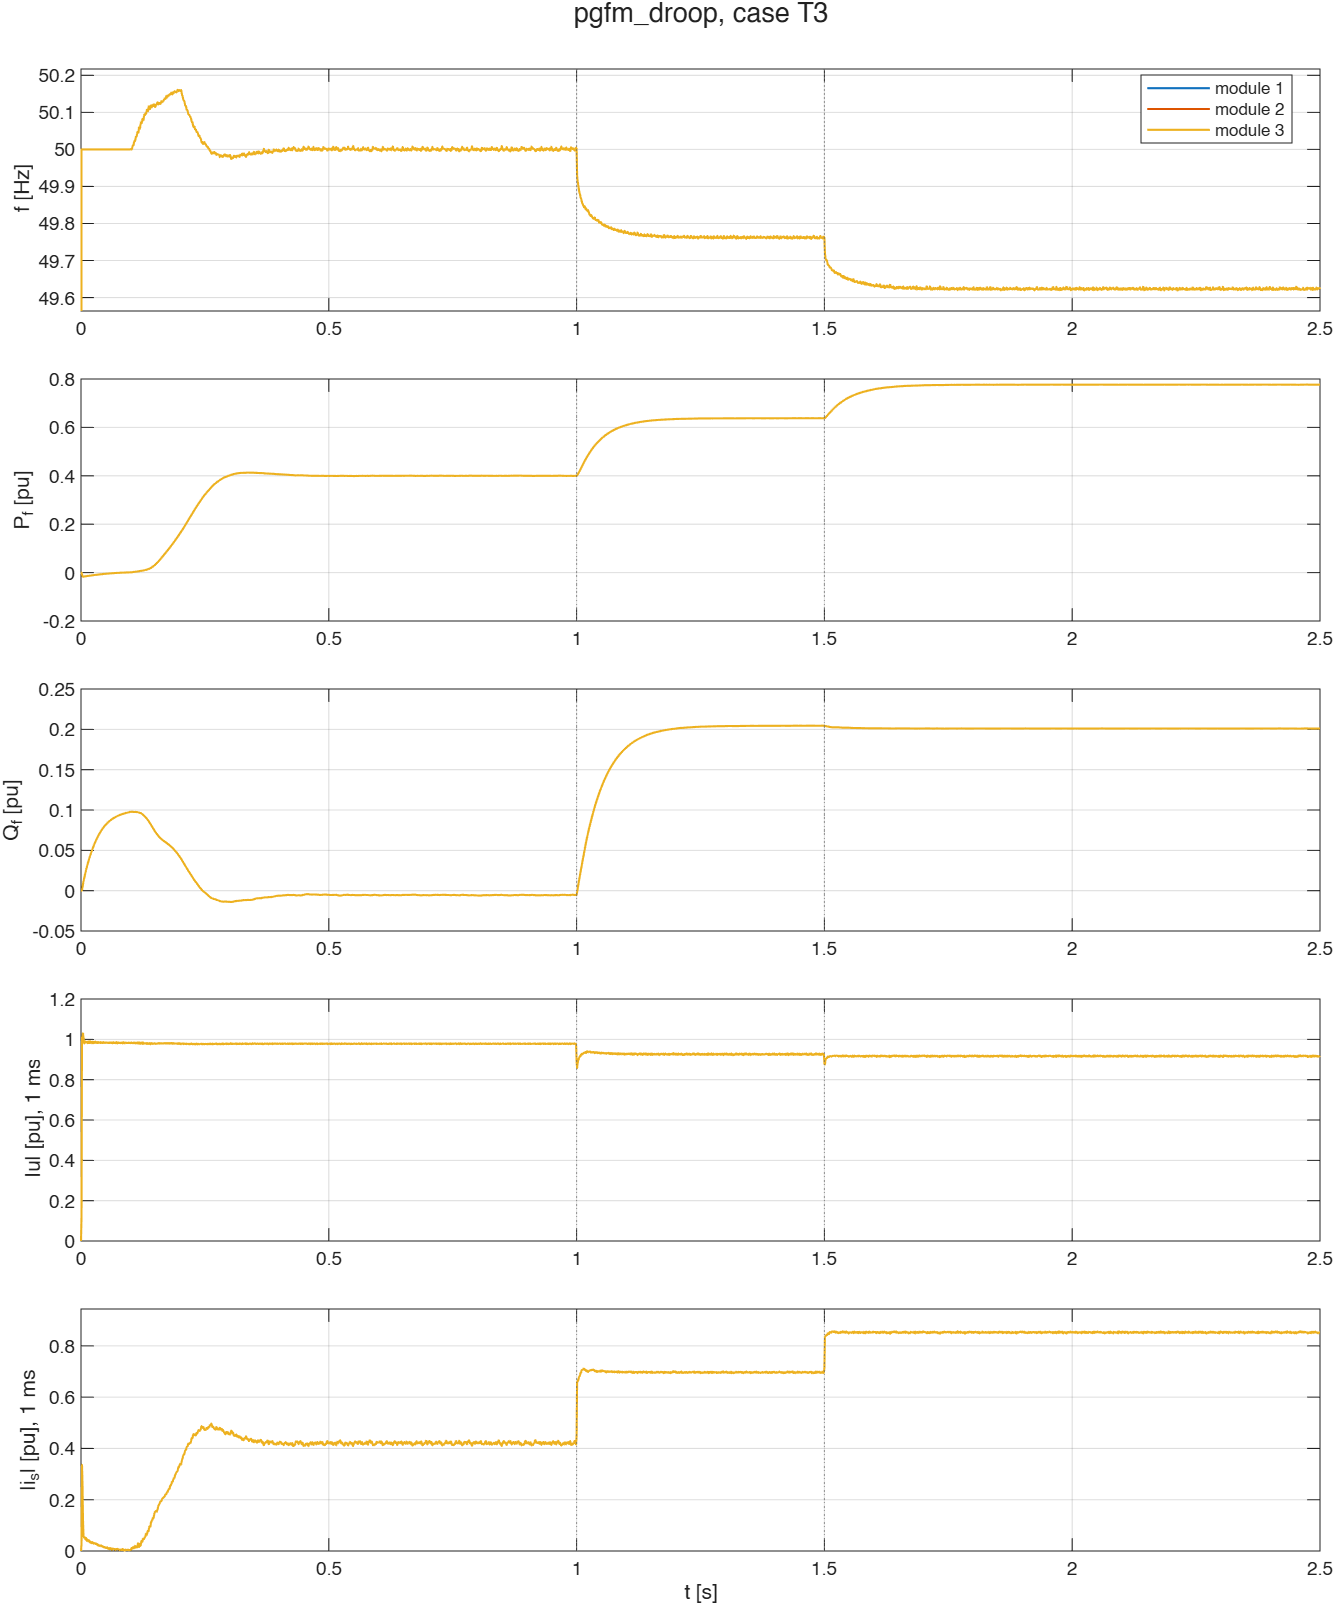
\includegraphics[width=0.78\textwidth]{figures/pgfm_droop_T3.png}
	\captionsetup{width=0.92\textwidth, font=small}
	\caption[Tests T2 and T3 on the companion model.]{Tests T2 and T3 on \code{pgfm\_droop}: start on the grid, loss of the grid at \SI{1.0}{s}, load step of +\SI{150}{\kilo\watt} at \SI{1.5}{s}. From the top: frequency of the phase generators, filtered active and reactive power, bus voltage and converter current (magnitudes, \SI{1}{ms} averages); the three modules overlap.}
	\label{fig:t3}
\end{figure}

\begin{figure}[H]
	\centering
	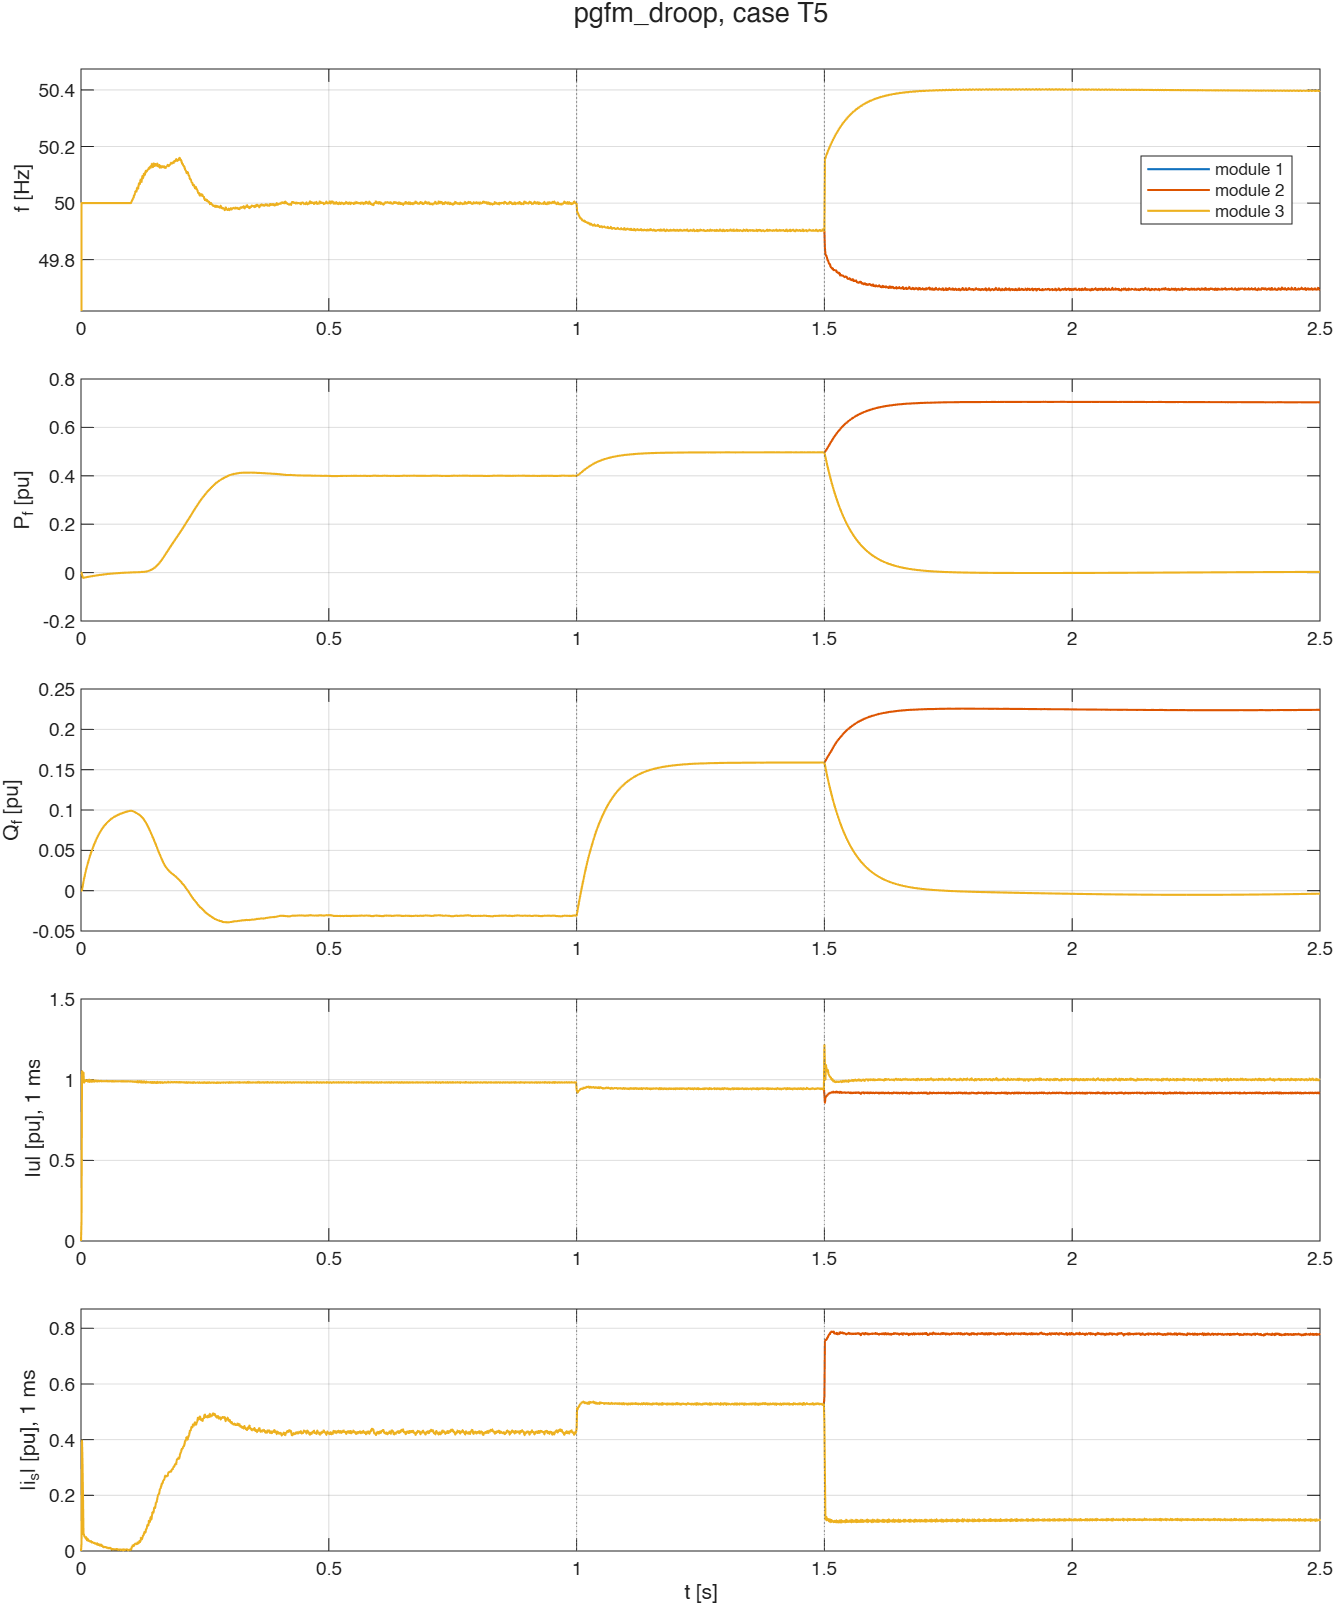
\includegraphics[width=0.78\textwidth]{figures/pgfm_droop_T5.png}
	\captionsetup{width=0.92\textwidth, font=small}
	\caption[Test T5 on the companion model.]{Test T5 on \code{pgfm\_droop}: \SI{450}{\kilo\watt} + \SI{150}{\kilo\var}, loss of the grid at \SI{1.0}{s}, trip of module 3 at \SI{1.5}{s}; after the trip module 3 runs alone at no load (\SI{50.4}{Hz}).}
	\label{fig:t5}
\end{figure}

\subsection{Version 2 and later}

Secondary control (frequency and voltage restoration in the island by the plant controller, or by distributed averaging \cite{simpsonporco2015}); resynchronization and reconnection; fault ride-through as grid-forming units with the current limitation of \cite{kiel_curlim} (test T6: FRT test 25.4 on the grid, current below \SI{1.2}{pu}, recovery, synchronism); angle droop on the PTP time \cite{golsorkhi2017} with the frequency droop as fallback if the time is lost; dVOC as comparison \cite{colombino2019}; the tertiary layer by online feedback optimization \cite{hauswirth2024}.

% =============================================================
\section{Common mode of modules on one battery}
\label{sec:cm}

\subsection{Where the common-mode voltage comes from}

The common-mode voltage of a two-level bridge, measured from the midpoint of its DC link, is the average of the three leg voltages, $v\ped{cm} = (v_{a0} + v_{b0} + v_{c0})/3 \in \{\pm u\ped{dc}/2, \pm u\ped{dc}/6\}$: at every commutation it jumps by $u\ped{dc}/3$, \SI{394}{V} at \SI{1183}{V}. Its low-frequency part is the zero-sequence voltage that the modulator adds to the references: the min--max injection of the space vector modulation is a triangle at three times the fundamental with a peak of a quarter of the phase amplitude, i.e.\ about \SI{114}{V} at \SI{150}{Hz} at full modulation. The simulation of Section~\ref{sec:hfsim} gives \SI{113}{V} at \SI{150}{Hz} (in the IT case \SI{10}{V} on the battery and \SI{103}{V} on the LV star point).

Each module pushes its common-mode voltage through its common-mode inductance. For the three-phase inductor of the model (Appendix~\ref{sec:files}), the zero-sequence inductance $L_0$ is per phase; the total common-mode current $i\ped{cm} = i_a + i_b + i_c$ of a module sees $L_0/3 = \SI{168}{\micro\henry}$ (leakage included).

\subsection{Circulating current between modules}

On one battery and one AC bus without transformers the modules form loops in which only the difference of their common-mode voltages acts (Figure~\ref{fig:cmloop}): the zero-sequence circulating current
\begin{equation}
	\frac{2L_0}{3}\,\frac{\dif i\ped{zs}}{\dif t} = v\ped{cm,1} - v\ped{cm,2}
	\label{eq:zscc}
\end{equation}
does not reach the grid and is not seen by a current loop in the $dq$ frame, but it loads the semiconductors and the chokes. Two sources matter:

\begin{itemize}[nosep]
	\item \textbf{different references.} The \SI{150}{Hz} zero-sequence voltage depends on the reference of each module \cite{zhu2017}: \SI{10}{\percent} of difference in the modulation (11~V at \SI{150}{Hz}) drives \SI{36}{A} through the \SI{337}{\micro\henry} of the loop, i.e.\ \SI{12}{A} per phase. With equal sharing (control V1) the references are close and this term is small; in transients, or with modules at different set-points as in the present scenario, it is not;
	\item \textbf{misaligned carriers.} With the carriers shifted, the common-mode pulses of the modules no longer coincide: half a carrier period of shift gives a ripple of about \SI{70}{A} peak to peak at the switching frequency. Interleaved carriers reduce the ripple seen by the grid \cite{modularity_note} but maximize this current: in parallel on one DC link, aligned carriers are the default.
\end{itemize}

\begin{figure}[H]
	\centering
	\begin{circuitikz}[european, font=\footnotesize, scale=0.95, transform shape]
		% modules: common-mode sources (referred to the DC midpoint) and common-mode chokes
		\draw (0,0) to[V, l=$v\ped{cm,1}$] (0,2.2) to[L, l=$L_0/3$] (0,4.4);
		\draw (2.8,0) to[V, l_=$v\ped{cm,2}$] (2.8,2.2) to[L, l_=$L_0/3$] (2.8,4.4);
		\draw (0,4.4) -- (8.4,4.4);
		\draw (0,0) -- (8.4,0);
		\node[above] at (1.4,4.4) {LV bus (common-mode node)};
		\node[below] at (1.4,0) {DC link midpoint (one battery)};
		% earth paths: AC side above, DC side below
		\draw (6.2,4.4) to[C, l=$3C\ped{ac}$] (6.2,2.2);
		\draw (8.4,4.4) to[R, l=$r\ped{star}$] (8.4,2.2);
		\draw (6.2,2.2) to[C, l=$2C\ped{pole}$] (6.2,0);
		\draw (8.4,2.2) to[R, l=$r\ped{gnd}/2$] (8.4,0);
		\draw (6.2,2.2) -- (8.4,2.2) -- (9.3,2.2) node[ground] {};
		\node[font=\scriptsize] at (7.3,2.45) {earth};
		% currents
		\draw[->, thick, red!70!black] (1.05,1.594) arc[start angle=-120, end angle=200, radius=0.7];
		\node[red!70!black] at (1.4,2.2) {$i\ped{zs}$};
		\draw[->, thick, blue!70!black, dashed] (5.3,3.9) -- (5.3,0.5);
		\node[blue!70!black, left] at (5.3,2.2) {$i\ped{e}$};
	\end{circuitikz}
	\captionsetup{width=0.9\textwidth, font=small}
	\caption[Common-mode paths of modules on one battery.]{Common-mode paths of modules on one battery (lumped, one source per module referred to the DC midpoint). Red: circulating current between the modules; blue: current to earth through the parasitic capacitances (Section~\ref{sec:earthing}).}
	\label{fig:cmloop}
\end{figure}

\subsection{PWM carriers aligned to the PTP time}

The alignment needs a common time in every module. IEEE 1588 (PTP) on a local network with hardware time stamps and PTP-aware switches keeps the clocks within some tens to a few hundred nanoseconds. With \SI{100}{ns} of residual shift each common-mode edge leaves $\SI{394}{V}\times\SI{100}{ns} \simeq \SI{39}{\micro\volt\second}$ on \SI{337}{\micro\henry}, about \SI{0.1}{A}: negligible. Without a common time, even good crystals drift apart: \SI{1500}{ppm} (module 2 of the model) loses half a carrier period in \SI{83}{ms}, \SI{50}{ppm} in \SI{2.5}{s}. The same time base gives the clocks of the droop (Section~\ref{sec:clock}) and the time stamps of the measurements.

\subsection{Measures in the model and next steps}

\begin{itemize}[nosep]
	\item keep the carriers aligned (\code{pwm\_phase\_shift\_modN} = 0) and the alignment loop of \code{global timing} on; run once with the alignment off to see the drift and the circulating current;
	\item the same modulator and the same zero-sequence injection in all modules; the term \code{u\_cm\_comp\_modN} must be checked against (\ref{eq:zscc}): different values between the modules create a \SI{150}{Hz} circulating current;
	\item log $i\ped{cm,k} = i_a + i_b + i_c$ of every module (a sum block per module, no new physical block);
	\item version 2: a loop per module on $i\ped{cm,k}$ acting on its zero-sequence voltage, PI plus resonant terms at 150 and \SI{450}{Hz} \cite{kiel_zscc}, or the modulation of \cite{zhu2017}.
\end{itemize}

% =============================================================
\section{Earthing of an industrial BESS and HF parasitics}
\label{sec:earthing}

\subsection{Earthing schemes}

The common-mode voltage of the bridges has to close somewhere: through the parasitic capacitances to earth of the DC side (battery, cables) and of the AC side (transformer winding, cables, AC nodes of the modules). Where it appears depends on which side is held to earth:

\begin{itemize}[nosep]
	\item \textbf{LV star point solidly earthed (TN)}, battery floating: the AC side is fixed to earth, so the battery carries the whole common-mode voltage of the bridges with respect to earth. Every cell, its insulation towards the racks and the cooling plates, and the cables see steps of $u\ped{dc}/3$ at the switching frequency; the earth current through the capacitance of the battery is the largest of all cases. This was the scheme of the model before November 2026.
	\item \textbf{LV side not earthed (IT), battery referenced to earth through a high impedance}: the common-mode voltage divides on the capacitances of the two sides; the battery, much larger than the AC side, stays almost still and the LV winding carries the common mode. It is the scheme of the industrial BESS with a power conversion system and an LV/MV transformer: the LV winding and everything galvanically connected to it (bridges, DC links, battery) form one IT system, with an insulation monitor (first fault signalled, not tripped) and residual current monitoring.
	\item \textbf{high-resistance earthing (HRG) of the LV star}: a resistor limits the first-fault current (here \SI{1.7}{A}) and makes it detectable; below the corner frequency $1/(2\pi r\ped{star} C)$ (\SI{2.1}{kHz} here) the star point is held to earth, so the \SI{150}{Hz} common mode goes back onto the battery, and the resistor carries a permanent common-mode current.
\end{itemize}

The transformer between the LV system and the MV network should be an inverter-duty unit with an earthed electrostatic screen between the windings: the common-mode current of the LV system then closes locally and is not coupled into the MV network, whose neutral treatment is the one of the network operator.

\subsection{Parasitic capacitances and earthing resistances in the model}

Table~\ref{tab:gnd} gives the values now in \code{init\_model.m} (\code{param.gnd}); Figure~\ref{fig:cmloop} shows where they are. The battery side is the network drawn in \code{battery\_1/HF and Ground Network}: from each pole a capacitor with its series resistance and an earthing resistor to earth. The AC side has the three phase capacitances lumped at the star point of the LV winding of the emulator transformer (\code{grid/grid\_emulator/3ph\_Dyg\_ssc}): the block \code{C\_lv\_earth} ($3C\ped{ac}$ with $r = r\ped{ac,hf}/3$) in parallel with \code{R\_star}. At the frequencies of interest the star point and the phases have the same common-mode voltage, and the lumped form costs two blocks less.

\begin{table}[H]
	\centering
	\captionsetup{width=0.9\textwidth, font=small}
	\caption{HF parasitics and earthing in \code{param.gnd}.}
	\label{tab:gnd}
	\rowcolors{2}{tableShade}{white}
	\footnotesize
	\begin{tabularx}{\textwidth}{@{} l l X @{}}
		\toprule
		\textbf{Field} & \textbf{Value} & \textbf{Origin} \\
		\midrule
		\code{c\_batt\_pole} & \SI{150}{nF} & cells to racks and cooling plates (about \SI{1}{nF} per prismatic cell of \SI{280}{\ampere\hour} through its insulation film), DC cables and busbars: about \SI{0.3}{\micro\farad} for a \SI{250}{\kilo\watt\hour} string, half per pole; it scales with the strings (about \SI{0.6}{\micro\farad} per pole for \SI{1}{MWh}) \\
		\code{r\_batt\_hf} & \SI{10}{\ohm} & series resistance of that path: earth conductors, skin effect, losses of the common-mode cores; it damps the common-mode resonance \\
		\code{r\_gnd\_pole} & \SI{100}{\kilo\ohm} & symmetric high-resistance reference of the poles: first-fault current $u\ped{dc}/r = \SI{12}{mA}$, \SI{7}{W} of losses; with an IMD, \SI{1}{\mega\ohm} or more (the IMD sees $r/2$) \\
		\code{c\_ac\_phase} & \SI{10}{nF} & LV winding to core and screen, LV cables, AC nodes of the IGBT modules to the heatsinks, per phase \\
		\code{r\_ac\_hf} & \SI{10}{\ohm} & series resistance of that path, per phase \\
		\code{r\_star} & \SI{1}{\giga\ohm} & IT (not earthed); \SI{230}{\ohm} for high-resistance earthing (\SI{1.7}{A}); \SI{0.1}{\ohm} for TN \\
		\bottomrule
	\end{tabularx}
	\rowcolors{1}{white}{white}
\end{table}

With these values the capacitive divider gives the battery $C\ped{ac,tot}/(C\ped{ac,tot} + C\ped{dc,tot}) = 30/330 = \SI{9.1}{\percent}$ of the common-mode voltage in the IT case. The common-mode loop (the chokes of the three modules in parallel, about \SI{56}{\micro\henry}, the zero-sequence leakage of the transformer and the \SI{27}{nF} of the two capacitances in series) resonates near \SI{100}{kHz}; with $t\ped{c} = \SI{1}{\micro s}$ the model resolves it with about ten steps per period, so the amplitude of that ringing is indicative only, while the \SI{150}{Hz} and the switching-frequency components are reliable.

\subsection{Simulation of the three schemes}
\label{sec:hfsim}

The script \path{parallel_of_GFMs/earthing_cases.m} runs the model to \SI{0.3}{s} for the three values of $r\ped{star}$, with the Simscape log of the earth paths, and evaluates the last three grid periods (Table~\ref{tab:hfres}, Figure~\ref{fig:hfcases}); the operating point is the one of the scenario, \SI{734}{\kilo\watt} into the battery at \SI{1183}{V}.

\begin{table}[H]
	\centering
	\captionsetup{width=0.92\textwidth, font=small}
	\caption[Earthing schemes: simulation results.]{Earthing schemes: voltages to earth and current to earth, last three grid periods of a run to \SI{0.3}{s} (\SI{734}{\kilo\watt} into the battery at \SI{1183}{V}). \SI{150}{Hz}: amplitude of that component; bands: rms value of the spectrum of the window in the band.}
	\label{tab:hfres}
	\rowcolors{2}{tableShade}{white}
	\small
	\begin{tabular}{@{} l r r r @{}}
		\toprule
		 & \textbf{IT} & \textbf{HRG} & \textbf{TN} \\
		 $r\ped{star}$ & \SI{1}{\giga\ohm} & \SI{230}{\ohm} & \SI{0.1}{\ohm} \\
		\midrule
		DC+ to earth, peak to peak [V] & 91 & 410 & 1158 \\
		battery (DC midpoint) to earth, \SI{150}{Hz} [V] & 10 & 112 & 113 \\
		LV star point to earth, peak to peak [V] & 830 & 607 & 3 \\
		LV star point to earth, \SI{150}{Hz} [V] & 102 & 7 & 0 \\
		current to earth, rms [A] & 0.64 & 0.71 & 4.41 \\
		current to earth, peak [A] & 2.6 & 2.7 & 15.7 \\
		\quad band 0--\SI{2}{kHz}, rms [mA] & 3 & 24 & 24 \\
		\quad band 2--\SI{20}{kHz}, rms [A] & 0.20 & 0.46 & 3.90 \\
		\quad band 20--\SI{500}{kHz}, rms [A] & 0.60 & 0.54 & 2.06 \\
		current in $r\ped{star}$, rms [A] & 0 & 0.46 & 4.41 \\
		losses in $r\ped{star}$ [W] & 0 & 49 & 2 \\
		\bottomrule
	\end{tabular}
	\rowcolors{1}{white}{white}
\end{table}

\begin{figure}[H]
	\centering
	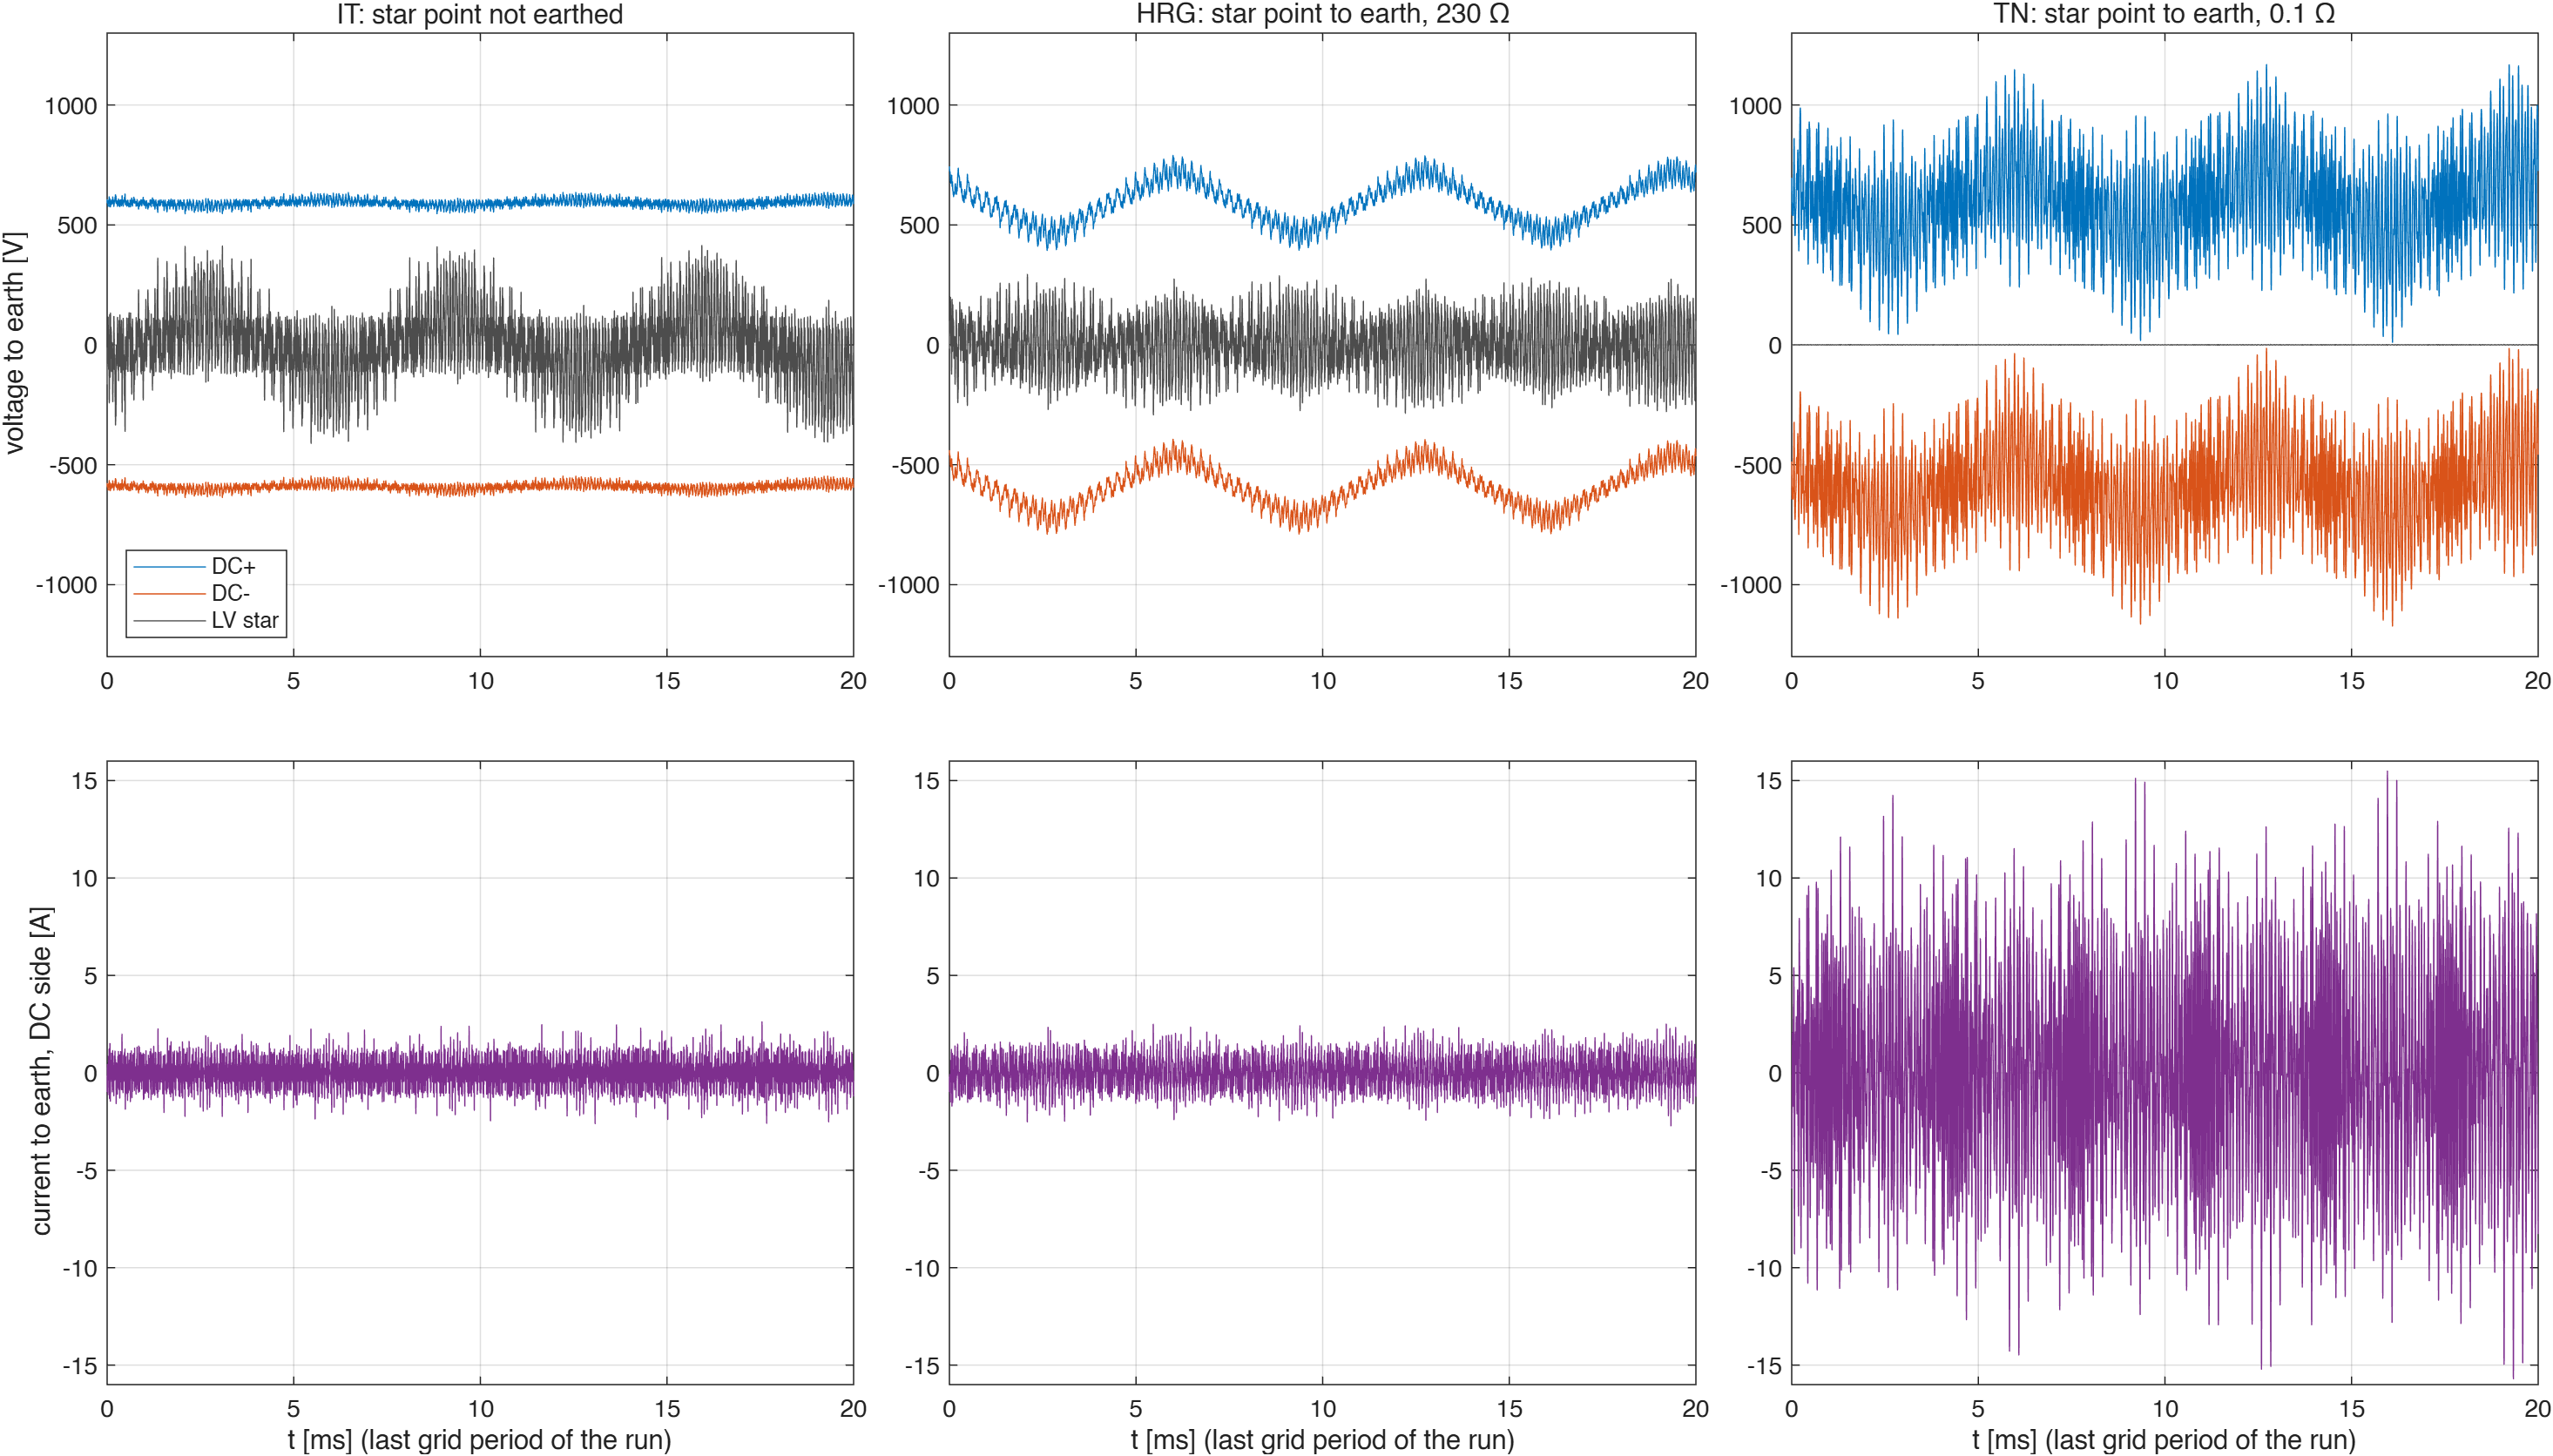
\includegraphics[width=\textwidth]{figures/hf_cases.png}
	\captionsetup{width=0.92\textwidth, font=small}
	\caption[Earthing schemes: voltages to earth and current to earth.]{The three earthing schemes, last grid period of the run: voltages to earth of DC+, DC$-$ and of the LV star point (top), current to earth of the DC side (bottom). Script \code{earthing\_cases.m}.}
	\label{fig:hfcases}
\end{figure}

\begin{itemize}[nosep]
	\item \textbf{IT.} The battery poles move by \SI{91}{V} peak to peak, mostly at the switching frequency and in the ringing of the common-mode loop; at \SI{150}{Hz} the battery has \SI{10}{V}, i.e.\ the \SI{9.1}{\percent} of the capacitive divider, and the LV star point carries the rest. The current to earth, \SI{0.64}{A} rms, is almost all above \SI{2}{kHz}.
	\item \textbf{HRG.} Below the corner frequency the star point is held to earth: the \SI{150}{Hz} common mode moves entirely onto the battery (\SI{112}{V}, poles \SI{410}{V} peak to peak), while the HF still divides on the capacitances. The resistor carries \SI{0.46}{A} rms of common-mode current (\SI{49}{W}): it counts in its rating, and the first-fault detection must tell it from a fault current.
	\item \textbf{TN.} The battery carries the whole common-mode voltage of the bridges: the poles swing by \SI{1158}{V} peak to peak, with steps of $u\ped{dc}/3 = \SI{394}{V}$ at every commutation that stress the insulation between the cells and the racks and cooling plates (against \SI{36}{V} steps in the IT case). The current to earth is \SI{4.4}{A} rms (\SI{15.7}{A} peak), seven times the IT case, through the battery insulation and the earth conductors.
\end{itemize}
The same current flows on the DC side and on the AC side, since it goes from one to the other through earth. The values above \SI{20}{kHz} contain the ringing of the common-mode loop, resolved with about ten solver steps per period: they are indicative.

\subsection{Insulation monitoring (IMD)}

In an IT system the first insulation fault does not trip anything: it must be signalled and removed before a second fault on another pole or phase turns it into a short circuit. The insulation monitor (IEC 61557-8 \cite{iec61557_8}) is connected between the system and earth, superimposes a measuring signal and computes the insulation resistance. For a BESS it must be of the type for \emph{IT AC systems with galvanically connected DC circuits}, since the LV winding, the bridges and the battery are one system, and it must tolerate the leakage capacitance of the system (here \SI{0.33}{\micro\farad}; several microfarads for a large plant) and the common-mode voltage of the converters. One IMD per galvanically connected system: two IMDs on the same system disturb each other.

The symmetric earthing resistors of the battery and the IMD do the same job in two ways: the resistors fix the potential of the poles and let a simple voltage measurement detect the first fault (a fault on DC+ brings DC+ to earth potential and DC$-$ to $-u\ped{dc}$); the IMD measures the insulation directly. With both, the IMD sees $r\ped{gnd}/2$ as a permanent insulation fault, so the resistors must be much larger than the IMD threshold, or left out. In the model $r\ped{gnd} = \SI{100}{\kilo\ohm}$ gives the poles a defined potential; the real value is a choice of the protection concept.

\subsection{Residual current monitoring unit (RCMU)}
\label{sec:rcmu}

\paragraph{What it is.} An RCMU measures the \emph{residual current}: the sum of the currents of all live conductors of a circuit, which is zero unless part of the current returns through earth. The conductors pass together through one magnetic core (a core-balance or summation current transformer); the core sees only their sum,
\begin{equation}
	i_\Delta = \sum_k i_k = -\,i\ped{earth},
	\label{eq:residual}
\end{equation}
three phases on the AC side, DC+ and DC$-$ on the DC side. Unlike an RCD, which opens its own contacts, the RCMU is a measuring function inside the converter: its signal goes to the control and protection of the converter, which opens the converter contactor. With power converters it must be of \emph{type B}: it measures smooth DC and AC residual currents up to the kilohertz range (a flux-gate sensor), because an insulation fault behind a rectifying bridge gives a DC residual current that saturates the core of an ordinary (type A) device.

\paragraph{Why a BESS needs it.} The IMD finds the slow degradation of the insulation; the RCMU finds the faults that appear at once, as a step of the residual current, and it measures what the IMD cannot: the capacitive leakage current that the common-mode voltage drives through the parasitic capacitances. For the transformerless PV inverters the rule is in IEC 62109-2 and VDE V 0126-1-1 \cite{iec62109_2, vde0126}, and it is often taken over for battery converters: disconnection when the continuous residual current exceeds \SI{300}{mA} (converters up to \SI{30}{\kilo\VA}) or \SI{10}{mA} per \si{\kilo\VA} (larger converters), and on sudden steps of 30, 60 and \SI{150}{mA} within 0.3, 0.15 and \SI{0.04}{s}. The step thresholds catch a fault current added on top of the capacitive leakage, whatever its size.

\paragraph{Where.} One summation transformer on the AC side of each PCS (the three phases, the star point of the IT system is not a conductor of the circuit), and one on the DC cables of each battery string (DC+ and DC$-$); Figure~\ref{fig:rcmu}. The AC one sees every earth current of the PCS; the DC one tells which string leaks.

\paragraph{What the model says.} The currents to earth of Table~\ref{tab:hfres} are the capacitive residual current that an RCMU of this plant sees without any fault; the AC and the DC summation transformers see the same current. Below \SI{2}{kHz} (type-B devices are specified up to about \SI{1}{kHz}) it is \SI{3}{mA} in the IT scheme and \SI{24}{mA} with the star point earthed, far from the continuous threshold (\SI{2.8}{A} for a module of \SI{278}{\kilo\VA}). Most of it is above the switching frequency: \SI{0.20}{A} in the 2--\SI{20}{kHz} band in the IT scheme against \SI{3.9}{A} in the TN scheme, which matters for devices with an extended bandwidth and for the EMC of the plant. In the earthed schemes the low-frequency part grows with the capacitance of the battery (ten times for some MWh), in the IT scheme it stays limited by the small capacitance of the AC side. A fault can be simulated by a resistor with a switch from one pole to earth: the step of $i_\Delta$ is the quantity to compare with the thresholds.

\begin{figure}[H]
	\centering
	\begin{tikzpicture}[font=\footnotesize, >=Latex,
		gb/.style={draw, thick, rounded corners=2pt, align=center, fill=gray!10},
		meas/.style={draw, thick, rounded corners=2pt, align=center, fill=yellow!15, font=\scriptsize}]
		% earth bar
		\draw[very thick] (-0.4,-3.0) -- (12.6,-3.0) node[right] {PE};
		% battery
		\node[gb, minimum width=1.5cm, minimum height=2.6cm] (bat) at (0.4,0) {battery\\string};
		\draw[thick] (1.15,0.9) -- (5.0,0.9) node[pos=0.2, above, font=\scriptsize] {DC+};
		\draw[thick] (1.15,-0.9) -- (5.0,-0.9) node[pos=0.2, above, font=\scriptsize] {DC$-$};
		% DC summation transformer
		\draw[thick, fill=yellow!40, fill opacity=0.5] (3.4,0) ellipse (0.22 and 1.25);
		\node[meas] at (3.4,1.75) {RCMU DC\\type B};
		% PCS
		\node[gb, minimum width=2.2cm, minimum height=2.6cm] (pcs) at (6.1,0) {PCS module\\bridge, $L$, $L_0$,\\$C\ped{F}$};
		% AC lines
		\foreach \y in {0.6,0,-0.6} { \draw[thick] (7.2,\y) -- (10.3,\y); }
		\draw[thick, fill=yellow!40, fill opacity=0.5] (8.6,0) ellipse (0.22 and 0.95);
		\node[meas] at (8.6,1.45) {RCMU AC\\type B};
		% transformer
		\draw[thick] (10.75,0) circle (0.45);
		\draw[thick] (11.4,0) circle (0.45);
		\draw[thick, dashed] (11.07,-0.75) -- (11.07,0.75);
		\node[font=\scriptsize, align=center] at (11.1,1.25) {LV/MV, earthed\\screen};
		\draw[thick] (11.85,0) -- (12.6,0) node[right] {MV};
		% screen to earth
		\draw (11.07,-0.75) -- (11.07,-1.05) -- (12.1,-1.05) -- (12.1,-3.0);
		% LV star point with IMD
		\draw (10.75,-0.45) -- (10.75,-1.5);
		\node[meas, minimum width=0.9cm] (imd) at (10.75,-1.8) {IMD};
		\draw (imd.south) -- (10.75,-3.0);
		% parasitic capacitances (dashed) and earthing resistor of the poles, drawn on DC- (the same on DC+)
		\draw (1.55,-0.9) to[R, l_={\scriptsize $r\ped{gnd}$}] (1.55,-3.0);
		\draw[dashed] (2.4,-0.9) to[C, l={\scriptsize $C\ped{pole}$}] (2.4,-3.0);
		\node[font=\scriptsize, align=center] at (1.95,-3.45) {(the same on DC+)};
		\draw[dashed] (6.1,-1.3) to[C, l={\scriptsize $C\ped{ac}$}] (6.1,-3.0);
		\draw[dashed] (9.6,-0.6) to[C, l_={\scriptsize $C\ped{ac}$}] (9.6,-3.0);
		% insulation fault between the summation transformer and the PCS
		\draw[red!70!black, thick] (4.5,-0.9) to[R, l={\scriptsize $R\ped{fault}$}, color=red!70!black] (4.5,-3.0);
		\draw[->, red!70!black, thick] (4.15,-1.45) -- (4.15,-2.45) node[midway, left, font=\scriptsize] {$i\ped{f}$};
	\end{tikzpicture}
	\captionsetup{width=0.92\textwidth, font=small}
	\caption[RCMU and IMD in a BESS with an IT LV system.]{RCMU and IMD in a BESS with an IT LV system (one PCS and one string shown). The summation transformers see the sum of the currents of their conductors, i.e.\ the current that returns through earth: the capacitive leakage through $C\ped{pole}$ and $C\ped{ac}$ (dashed) and the current of an insulation fault (red). The IMD sits between the LV system and earth; the screen of the transformer keeps the common-mode current away from the MV network.}
	\label{fig:rcmu}
\end{figure}

% =============================================================
\section{Three-level modules (future)}
\label{sec:3l}

A three-level module (NPC or T-type) changes the common mode and the earthing in the right direction and adds one constraint:

\begin{itemize}[nosep]
	\item the common-mode steps are $u\ped{dc}/6$ instead of $u\ped{dc}/3$: half the $\dif v/\dif t$ seen by the parasitic capacitances, half the HF earth current for the same switching speed, smaller common-mode chokes;
	\item each module has a neutral point in its split DC link; one high-resistance earthing at a neutral point gives the reference of the IT system without the two pole resistors;
	\item the neutral-point balance is done with the zero-sequence voltage or with the redundant small vectors: in modules on one battery this changes the zero-sequence voltage of each module and drives the circulating current of Section~\ref{sec:cm}. The balancing of the modules must be coordinated (same strategy, aligned carriers) or the circulating current controlled;
	\item the control V1 does not change; the library already has a three-level T-type power stage as a Simscape component (\path{+afe_ttype_ssc/afe_three_level_ttype_lcl.ssc}), so the step is the power stage, the modulator and the neutral-point loop.
\end{itemize}

% =============================================================
\section{Conclusions and next steps}
\label{sec:conclusions}

The model now has the parasitic capacitances and the earthing resistances of an industrial BESS, with the LV side not earthed and the battery referenced to earth through high resistances; the three earthing schemes can be compared with one parameter, and the simulation confirms that the battery stays quiet only when the LV star point is not held to earth. For the power sharing the control V1 is a droop control equivalent to a virtual synchronous machine, with a virtual impedance in front of a voltage loop on the filter capacitor and of the existing current loop: it shares the active power exactly, works the same on the grid and in the island, and needs the PTP time already modelled to remove the effect of the clock errors on the sharing. It is the droop mode of the library block \code{grid\_forming\_dqctrl}; on the companion model \code{pgfm\_droop} it passes the tests T0 to T5 and the black start, with the frequencies, voltages and sharing errors that the analysis predicts. The next steps are:

\begin{enumerate}[nosep]
	\item breaker and local load in \code{pgfm\_ctrl\_analysis} and the control V1 in its modules (route B), with the common-mode currents of the modules logged;
	\item version 2: secondary control of frequency and voltage, a slow correction of the reactive sharing by the plant controller, resynchronization, fault ride-through as grid-forming units (test T6), circulating-current loop;
	\item a battery sized for the three modules (and its parasitic capacitance), the initial voltage of the DC links;
	\item three-level modules.
\end{enumerate}

% =============================================================
\appendix
\section{Files}
\label{sec:files}

\begin{table}[H]
	\centering
	\captionsetup{width=0.9\textwidth, font=small}
	\caption{Files referred to in this note.}
	\label{tab:files}
	\rowcolors{2}{tableShade}{white}
	\small
	\begin{tabularx}{0.97\textwidth}{@{} >{\raggedright\arraybackslash}p{0.42\textwidth} X @{}}
		\toprule
		\textbf{File} & \textbf{Content} \\
		\midrule
		\multicolumn{2}{@{}p{\dimexpr0.97\textwidth-2\tabcolsep\relax}@{}}{\textbf{\code{grid-forming}, folder \path{parallel_of_GFMs/}}} \\
		\code{init\_model.m} & initialization, one \code{param} struct; \code{param.gnd} (Table~\ref{tab:gnd}); puts the folder of this note on the path \\
		\code{pgfm\_ctrl\_analysis.slx} & the model; \code{battery\_1/HF and Ground Network}, \code{grid/grid\_emulator/3ph\_Dyg\_ssc} (\code{R\_star}, \code{C\_lv\_earth}); the annotation \emph{Design note} at the top left opens this PDF \\
		\code{earthing\_cases.m} & the three earthing schemes of Section~\ref{sec:hfsim}: table and figure \\
		\path{power_sharing/init_pgfm_droop.m} & parameters and cases of the companion model (Section~\ref{sec:tests}) \\
		\path{power_sharing/build_pgfm_droop.m} & builds \code{pgfm\_droop.slx}, the companion model of route A: change the script, not the model \\
		\path{power_sharing/pgfm_droop_tests.m} & runs the cases, checks them and writes \path{results/<case>.txt}, \code{.png} \\
		\midrule
		\multicolumn{2}{@{}p{\dimexpr0.97\textwidth-2\tabcolsep\relax}@{}}{\textbf{\code{library}}} \\
		\path{masked_models/grid_forming/} & block \code{grid\_forming\_dqctrl} and its control \code{private/afe\_dq\_ctrl\_pwm.m} with the droop mode (\code{p.ctrl.droop = 1}); \code{grid\_forming\_param\_example.m} with the fields \code{droop\_*}; \code{test/grid\_forming\_droop\_test\_run.m} \\
		\path{foundation/pwr_electronics/+threephase_inductor/} & three-phase inductor: $L_0$ is the zero-sequence inductance per phase \\
		\path{foundation/pwr_electronics/+afe_ttype_ssc/} & three-level T-type power stage (Section~\ref{sec:3l}) \\
		\midrule
		\multicolumn{2}{@{}p{\dimexpr0.97\textwidth-2\tabcolsep\relax}@{}}{\textbf{\code{repositories-documentation}, folder \path{repos_doc/parallel_of_gfms/}}} \\
		\code{parallel\_of\_gfms.tex}, \code{.pdf} & this note \\
		\code{figures/hf\_cases.png} & Figure~\ref{fig:hfcases}, written by \code{earthing\_cases.m} \\
		\code{figures/pgfm\_droop\_T3.png}, \code{\_T5.png} & Figures~\ref{fig:t3} and~\ref{fig:t5}, written by \code{pgfm\_droop\_tests.m} \\
		\bottomrule
	\end{tabularx}
	\rowcolors{1}{white}{white}
\end{table}

% =============================================================
\begin{thebibliography}{99}
	\small
	\bibitem{rosso2021} R.~Rosso, X.~Wang, M.~Liserre, X.~Lu, and S.~Engelken, ``Grid-forming converters: control approaches, grid-synchronization, and future trends---a review,'' \emph{IEEE Open J. Ind. Appl.}, vol.~2, pp.~93--109, 2021, doi:10.1109/OJIA.2021.3074028.
	\bibitem{rosso2019} R.~Rosso, S.~Engelken, and M.~Liserre, ``Robust stability analysis of synchronverters operating in parallel,'' \emph{IEEE Trans. Power Electron.}, 2019, doi:10.1109/TPEL.2019.2897707.
	\bibitem{rosso2020} R.~Rosso, S.~Engelken, and M.~Liserre, ``Robust stability investigation of the interactions among grid-forming and grid-following converters,'' \emph{IEEE J. Emerg. Sel. Topics Power Electron.}, vol.~8, no.~2, pp.~991--1003, 2020, doi:10.1109/JESTPE.2019.2951091.
	\bibitem{zhou2022} W.~Zhou, A.~Pugliese, M.~Langwasser, and M.~Liserre, ``Sub-synchronous damping by battery storage system in grid forming control mode,'' in \emph{Proc. IEEE ECCE}, 2022, pp.~1--8, doi:10.1109/ECCE50734.2022.9947758.
	\bibitem{kiel_curlim} ``Current limitation strategy for grid-forming converters under symmetrical and asymmetrical grid faults,'' Kiel University, Chair of Power Electronics, record in the university repository MACAU, \url{https://macau.uni-kiel.de/receive/macau_mods_00001568}.
	\bibitem{zhu2017} R.~Zhu, M.~Liserre, Z.~Chen, and X.~Wu, ``Zero-sequence voltage modulation strategy for multiparallel converters circulating current suppression,'' \emph{IEEE Trans. Ind. Electron.}, vol.~64, no.~3, pp.~1841--1852, Mar. 2017, doi:10.1109/TIE.2016.2623259.
	\bibitem{kiel_zscc} ``Analysis and suppression of zero-sequence circulating current in multi-parallel converters,'' Kiel University, record in the university repository MACAU, \url{https://macau.uni-kiel.de/receive/macau_mods_00001642}.
	\bibitem{bolognani2013} S.~Bolognani and S.~Zampieri, ``A distributed control strategy for reactive power compensation in smart microgrids,'' \emph{IEEE Trans. Autom. Control}, vol.~58, no.~11, pp.~2818--2833, Nov. 2013, doi:10.1109/TAC.2013.2270317.
	\bibitem{bolognani2015} S.~Bolognani, R.~Carli, G.~Cavraro, and S.~Zampieri, ``Distributed reactive power feedback control for voltage regulation and loss minimization,'' \emph{IEEE Trans. Autom. Control}, vol.~60, no.~4, pp.~966--981, Apr. 2015, doi:10.1109/TAC.2014.2363931.
	\bibitem{hauswirth2024} A.~Hauswirth, Z.~He, S.~Bolognani, G.~Hug, and F.~D\"orfler, ``Optimization algorithms as robust feedback controllers,'' \emph{Annual Reviews in Control}, vol.~57, art.~100941, 2024, doi:10.1016/j.arcontrol.2024.100941.
	\bibitem{colombino2019} M.~Colombino, D.~Gro\ss, J.-S.~Brouillon, and F.~D\"orfler, ``Global phase and magnitude synchronization of coupled oscillators with application to the control of grid-forming power inverters,'' \emph{IEEE Trans. Autom. Control}, vol.~64, no.~11, pp.~4496--4511, Nov. 2019.
	\bibitem{simpsonporco2013} J.~W. Simpson-Porco, F.~D\"orfler, and F.~Bullo, ``Synchronization and power sharing for droop-controlled inverters in islanded microgrids,'' \emph{Automatica}, vol.~49, no.~9, pp.~2603--2611, 2013, doi:10.1016/j.automatica.2013.05.018.
	\bibitem{simpsonporco2015} J.~W. Simpson-Porco, Q.~Shafiee, F.~D\"orfler, J.~C. Vasquez, J.~M. Guerrero, and F.~Bullo, ``Secondary frequency and voltage control of islanded microgrids via distributed averaging,'' \emph{IEEE Trans. Ind. Electron.}, vol.~62, no.~11, pp.~7025--7038, Nov. 2015, doi:10.1109/TIE.2015.2436879.
	\bibitem{chandorkar1993} M.~C. Chandorkar, D.~M. Divan, and R.~Adapa, ``Control of parallel connected inverters in standalone AC supply systems,'' \emph{IEEE Trans. Ind. Appl.}, vol.~29, no.~1, pp.~136--143, Jan./Feb. 1993.
	\bibitem{guerrero2005} J.~M. Guerrero, L.~Garc\'ia de Vicu\~na, J.~Matas, M.~Castilla, and J.~Miret, ``Output impedance design of parallel-connected UPS inverters with wireless load-sharing control,'' \emph{IEEE Trans. Ind. Electron.}, vol.~52, no.~4, pp.~1126--1135, Aug. 2005.
	\bibitem{guerrero2011} J.~M. Guerrero, J.~C. Vasquez, J.~Matas, L.~Garc\'ia de Vicu\~na, and M.~Castilla, ``Hierarchical control of droop-controlled AC and DC microgrids---a general approach toward standardization,'' \emph{IEEE Trans. Ind. Electron.}, vol.~58, no.~1, pp.~158--172, Jan. 2011.
	\bibitem{zhong2011} Q.-C. Zhong and G.~Weiss, ``Synchronverters: inverters that mimic synchronous generators,'' \emph{IEEE Trans. Ind. Electron.}, vol.~58, no.~4, pp.~1259--1267, Apr. 2011.
	\bibitem{zhang2010} L.~Zhang, L.~Harnefors, and H.-P. Nee, ``Power-synchronization control of grid-connected voltage-source converters,'' \emph{IEEE Trans. Power Syst.}, vol.~25, no.~2, pp.~809--820, May 2010.
	\bibitem{darco2014} S.~D'Arco and J.~A. Suul, ``Equivalence of virtual synchronous machines and frequency-droops for converter-based microgrids,'' \emph{IEEE Trans. Smart Grid}, vol.~5, no.~1, pp.~394--395, Jan. 2014, doi:10.1109/TSG.2013.2288000.
	\bibitem{pogaku2007} N.~Pogaku, M.~Prodanovi\'c, and T.~C. Green, ``Modeling, analysis and testing of autonomous operation of an inverter-based microgrid,'' \emph{IEEE Trans. Power Electron.}, vol.~22, no.~2, pp.~613--625, Mar. 2007, doi:10.1109/TPEL.2006.890003.
	\bibitem{darco2015} S.~D'Arco, J.~A. Suul, and O.~B. Fosso, ``A virtual synchronous machine implementation for distributed control of power converters in SmartGrids,'' \emph{Electr. Power Syst. Res.}, vol.~122, pp.~180--197, May 2015, doi:10.1016/j.epsr.2015.01.001.
	\bibitem{paquette2015} A.~D. Paquette and D.~M. Divan, ``Virtual impedance current limiting for inverters in microgrids with synchronous generators,'' \emph{IEEE Trans. Ind. Appl.}, vol.~51, no.~2, pp.~1630--1638, Mar./Apr. 2015.
	\bibitem{golsorkhi2017} M.~S. Golsorkhi, D.~D.-C. Lu, and J.~M. Guerrero, ``A GPS-based decentralized control method for islanded microgrids,'' \emph{IEEE Trans. Power Electron.}, vol.~32, no.~2, pp.~1615--1625, Feb. 2017, doi:10.1109/TPEL.2016.2551265.
	\bibitem{ye2002} Z.~Ye, D.~Boroyevich, J.-Y. Choi, and F.~C. Lee, ``Control of circulating current in two parallel three-phase boost rectifiers,'' \emph{IEEE Trans. Power Electron.}, vol.~17, no.~5, pp.~609--615, Sept. 2002, doi:10.1109/TPEL.2002.802170.
	\bibitem{teodorescu2011} R.~Teodorescu, M.~Liserre, and P.~Rodr\'iguez, \emph{Grid Converters for Photovoltaic and Wind Power Systems}. Wiley-IEEE Press, 2011.
	\bibitem{afe_note} D.~Bagnara, \emph{Grid-forming and grid-following AFE blocks: two-level bridge with LCL filter, description and user guide}, pwr-control technical note, Rev.~00, October 2026, \path{repos_doc/grid_forming_following_afe}.
	\bibitem{gfm_note} D.~Bagnara, \emph{Grid-Forming Control in the Synchronous dq Frame: structure, continuous-time design and discrete implementation}, pwr-control technical note, Rev.~00, October 2026, \path{research/power_electronics/grid_forming_control}.
	\bibitem{modularity_note} D.~Bagnara, \emph{Modularity in Power Electronics: impact on grid power quality}, pwr-control report, October 2023, \path{repos_doc/modularity}.
	\bibitem{iec61557_8} IEC 61557-8, \emph{Electrical safety in low voltage distribution systems up to 1000~V a.c. and 1500~V d.c.\ -- Equipment for testing, measuring or monitoring of protective measures -- Part 8: Insulation monitoring devices for IT systems}.
	\bibitem{iec62109_2} IEC 62109-2, \emph{Safety of power converters for use in photovoltaic power systems -- Part 2: Particular requirements for inverters}.
	\bibitem{vde0126} VDE V 0126-1-1, \emph{Automatic disconnection device between a generator and the public low-voltage grid}.
	\bibitem{ieee1588} IEEE 1588, \emph{Standard for a Precision Clock Synchronization Protocol for Networked Measurement and Control Systems}.
\end{thebibliography}

\end{onehalfspace}
\end{document}
